

\section{Приближение функций \texorpdfstring{$\rr$}{равномерно}, в среднем и среднеквадратичном}
\sbs{1}{Приближение функций кусочно-линейными и  многочленами}
% 112 страница (4.7)

\textit{Носитель} функции -- дополнение к объдинению всех открытых множеств, на которых функция равна нулю, иначе -- замыкание множества точек, в которых функция не равна нулю. Получается носитель функции всегда замкнут и для функций на $\mathbb{Rn}$ компактнось носителя означает ограниченность. 

\begin{to_lem}
    Для непрерывной с компактным носителем $f(x) \colon \mathbb{R} \to \mathbb{R}$ и $t_n \to 0$ при $n \to \infty$, последовательность $f_n(x) = f(x + t_n) \rr f$.
\end{to_lem}

\begin{uproof}
Непрерывня функция с компактным носителем равномерно непрерывна, то есть
\begin{equation*}
    \forall \varepsilon > 0 \,  \exists \delta > 0 \, \forall x \in \mathbb{R},\, \forall t,\, \ 
    \left(
        |t| < \delta \ \Rightarrow \ |f(x-t) - f(x)| < \varepsilon,
    \right)
\end{equation*}
что можно интепретировать как равномерной сходимости $f(x-t_n) \rr f(x)$. 
\end{uproof}

% --------------------------------

\begin{to_thr}[]
    Для $|x| < 1$ и $\alpha \in \mathbb{R}$ $$(1+x)^\alpha = \sum_{n=0}^{\infty} \begin{pmatrix}
        a \\ n
    \end{pmatrix} x^n$$ с радиуом сходимости не менее $1$. 
\end{to_thr}

\begin{to_lem}
    $f(x) = \sqrt{x}$ можно равномерно приблизить многочленами на любом отрезке $[0,a]$.
\end{to_lem}

\begin{uproof}
    Заменой переменной $x = a -y$ сведем вопрос к приближению функции
    \begin{equation*}
        g(y) = \sqrt{a + \delta} \sqrt{1 - \frac{y}{a+\delta}},
    \end{equation*}
    который раскладывается по предыдущей лемме в степенной ряд при $|y| \leq a + \delta$, причём при $|y| \leq a$ ряд сходится равномерно, тогда $g(y)$ приближается многочленом на $[0, a]$, соответственно и $\sqrt{x}$ тоже. 
\end{uproof}


% --------------------------------

\begin{to_lem}
    $f(x) = |x|$ можно равномерно приблизить многочленами на любом отрезке $[-a,a]$.
\end{to_lem}

\begin{uproof}
Идея 
\end{uproof}

\begin{uproof}
    На отрезке $[0, a^2]$ приближаем $\sqrt{t}$ многочленом $|\sqrt{t} - P(t)| < \varepsilon$. Подставим $x = \sqrt{t}$, тогда на $x \in [0, a]$ верно $|x - P(x^2)| < \varepsilon$, что можно продолжить на $[-a, a]$, продолжая $x$ чётным образом как $|x|$: $\big| |x| - P(x^2) \bigg| < \varepsilon$. 
\end{uproof}

% --------------------------------

\begin{to_thr}
    Всякую непрерывную кусочно-линейную на отрезке $[a, b]$ функцию можно сколь угодно близко равномерно приблизить многочленом.
\end{to_thr}

\begin{uproof}
Если функция со скачком производной на $\Delta$, то $f(x) - \Delta/2 |x-x_i|$ будет уже без скачка, тогда кусочно-линейная представится в виде
\begin{equation*}
    f(x) = \sum_i c_i |x - x_i | + a x + b,
\end{equation*}
где каждое слагаемой уже приближаемо. 
\end{uproof}

Этого достаточно, чтобы приближать кусочно-линейные многочленами. Осталось понять, как приближать непрерывные на отрезке функции  кусочно-линейными. Определим
\begin{equation*}
    \varphi_\delta (x) = \left\{\begin{aligned}
        &0, & x < - \delta, \\
        & 1 - |x|/\delta, &|x| \leq \delta \\ 
        &0, & x > \delta.
    \end{aligned}\right.
\end{equation*}
Такая функция кусочно линейная, непрерывная, и её носитель -- $[-\delta, \delta]$.

% --------------------------------

\begin{to_lem}
    Для непрерывной $f \colon [0,1] \to \mathbb{R}$: $\sum\limits_{k = 0}^{m} f(k/m) \varphi_{1/m} (x - k/m) \rr f$.
\end{to_lem}

\begin{uproof}
Воспользуемся разбиением единицы
\begin{equation*}
    \sum_{k=0}^{m} \varphi_{1/m} (x - k/m) = 1.
\end{equation*}
Умножая это на $f(x)$ и вычитая $f_m(x)$, получаем
\begin{equation*}
    f(x) - f_m (x) = \sum_{k=0}^{m}  \left(
        f(x)- f(k/m)
    \right) \varphi_{1/m} (x-k/m).
\end{equation*}
При фиксированном $x$ в правой части слагаемые ненулевые только при $|x-k/m|<1/m$. Тогда правую часть оценим через модуль непрерывности 
\begin{equation*}
    \bigg| \sum_{k=0}^{m}  \left(
        f(x)- f(k/m)
    \right) \varphi_{1/m} (x-k/m) \bigg| \leq 
    \sum_{k=0}^{m}  \omega_f (1/m) \varphi_{1/m} (x-k/m) = \omega_f (1/m),
\end{equation*}
который стремится к нулю при $m \to \infty$ по непрерывности $f$. Напомним, что
\begin{equation*}
    \omega_f (\delta) = \sup \left\{
        \rho(f(x) - f(y)) \mid x, y \in M,\, \ \rho(x, y) < \delta.
    \right\}
\end{equation*}


\end{uproof}

% --------------------------------

\begin{to_thr}
    Всякую $f \colon [a_1, b_1] \times [a_n, b_n] \to \mathbb{R}$ можно сколь угодно близко
равномерно приблизить многочленом.
\end{to_thr}


\begin{uproof}
    Сначала масштабируем параллелепипед в единичный куб. Потом равномерно приближаем непрерывную функцию комбинацией произведений кусочно-линейных функций отдельных переменных:
\begin{equation*}
    f \colon  [0, 1]^n \mapsto \mathbb{R}, \hspace{5 mm} 
    f_m (x) = \sum_{k_1, \ldots, k_n} f\left(
        \frac{k_1}{m}, \ldots, \frac{k_n}{m}
    \right) \varphi_{1/m}\left(x_1 -\frac{k_1}{m}\right) \ldots \varphi_{1/m} \left(x_n - \frac{k_n}{m}\right).
\end{equation*}
     Потом их приближаем многочленами. 
\end{uproof}sw
\sbs{2}{Приближение \texorpdfstring{$2\pi$}{2pi}-периодических функций тригонометрическими многочленами}
% 115 страница (4.8)

\begin{to_thr}[теорема Вейерштрасса]
    Всякую непрерывную $2\pi$-периодичную $f \colon \mathbb{R} \to \mathbb{R}$ можно сколько угодно точно равномерно приблизить $T(x) = a_0 + \sum\limits_{k = 1}^{n}(a_k \cos(k x) + b_k \sin(k x)) $.
\end{to_thr}
 
\sbs{3}{* Алгебры непрерывных на компактах функций. Теорема Стоуна-Вейерштрасса}

\begin{to_def}
    $\mathcal{A} \subseteq C(x)$(-- непрерывные на компакте функции) называется \textit{алгеброй}, если она содержит константы ($\mathbb{R} \subseteq \mathcal{A}$) и топологически "замкнута" относительно операций $+$ и $\bullet$.
\end{to_def}

\begin{to_def}
    \textit{Алгебра разделяющая точки} --- $\forall a, b \in \mathbb{R},\, x=y \in X,\, \, \exists f \in A$ такая что $f(x)=a$, а $f(y) = b$.
\end{to_def}

\begin{to_thr}[теорема Стоуна-Вейерштрасса]
    Если $X$-метрический компакт, а алгебра $\mathcal{A}\in C(x)$ разделяет точки, \textbf{то} $\forall f \in C(x)$ можно сколь угодно точно равномерно приблизить функциями из $\mathcal{A}$.
\end{to_thr} 
\sbs{4}{Пространства \texorpdfstring{$L_p$}{Lp}. Неравенства Гёльдера и Минковского.}

\subsubsection*{Неравенства Гёльдера и Минковского}

\begin{to_def}
    \textit{Абсолютно интегрирумыми функциями} на измеримом $X \subseteq \mathbb{R}^n$ называют $f \colon X \mapsto \mathbb{R}$ с конечным интегралом $\int_X |f(x)| \d x$. \textit{Расстоянием}\footnote{
        В силу неравенства $|f(x) - g(x)| \leq |f(x)| + |g(x)|$ расстояние конечно.
    } между функциями $f$ и $g$ будем считать $\int_X |f(x)-g(x)| \d x$.
\end{to_def}

\begin{to_def}
    Обозначим через $L_1 (X)$ факторпространство  линейного пространства абсолютно интегрируемых функций по его линейному подпространству почти всюду равных нулю функций. То есть функции на $0$ расстоянии считаем равными. \textit{Нормой} будем считать
    \begin{equation*}
        \|f\|_1 = \int_X |f(x)| \d x.
    \end{equation*}
\end{to_def}

\begin{to_def}
    Для измеримого по Лебегу $X \subset \mathbb{R}^n$ и числа $p \geq 1$ \textit{факторпространство} измеримых по Лебегу функций на $X$ с конечной (полу)нормой
    \begin{equation*}
        \|f\|_p
        = 
        \left(
            \int_X |f|^p \d x
        \right)^{1/p},
    \end{equation*}
    по модулю функций равных нулю почти всюду,
    назовём $L_p (X)$.
\end{to_def}

\texttt{Очень хорошим, симметричным, актуальным для описания квантовой механики оказывается $L_2$ простран-\\ство, на котором естественно вводить скалярное произведение, его порождающее.} 

 \begin{to_def}
     В комплексном случае норма $L_2$ порождена \textit{скалярным произведением}
     \begin{equation*}
         (f, g) = \int_{-\infty}^{+\infty} f(x) \overline{g(x)} \d x
         \hspace{0.5cm} \longrightarrow \hspace{0.5cm}
         \|f\|_2 = \sqrt{(f, f)}.
     \end{equation*}
 \end{to_def}


\begin{to_thr}[Неравенство Гёльдера]
    Возьмём $p, \, q > 1$ такие, что $1/p + 1/q = 1$. Пусть $f \in L_p (X)$ и $g \in L_q(X)$. Тогда
    \begin{equation*}
        \int_X |fg| \d x \leq \|f\|_p \cdot \|g\|_q.
    \end{equation*}
\end{to_thr}

\begin{proof}[$\triangle$]
    Для доказательства достаточно проинтегрировать неравенство вида
    \begin{equation*}
        |fg| \leq \frac{|f|^p}{p} + \frac{|g|^q}{q}.
    \end{equation*}
    \red{Осталось получить само неравенство.}
\end{proof}

\begin{to_con}
    Для измеримых функций и чисел $p, \, q > 0$, таких что $1/p + 1/q = 1$, имеет место формула
    \begin{equation}
        \label{8_1}
        \|f\|_p = \sup \left\{
            \int_X fg \d x \ \bigg| \  \|g\|_q \leq 1
        \right\}.
    \end{equation}
\end{to_con}

\begin{proof}[$\triangle$]
По неравенству Гёльдера норма $f$ не менее супремума правой части \red{(?)}, более того равенство достигается при выборе
\begin{equation*}
    g(x) = \frac{\sign f(x) |f(x)|^{p-1}}{\|f\|_p^{p-1}}.
\end{equation*}
\end{proof}

\begin{to_def}
    Функция $f \colon V \mapsto \mathbb{R}$ на векторном пространство называется выпуклой, если для любых $x, \, y \in V$ и любого $t \in (0, 1)$ имеет место неравенство
    \begin{equation*}
        f ( (1-t) x + ty) \leq (1-t) f(x) + t f(y).
    \end{equation*}
    Функция называется \textit{строго выпуклой}, если неравенство строгое $\forall x \neq y$ и $t \in (0, 1)$. 
\end{to_def}

\begin{to_lem}
    Если в семействе функций $f_\alpha \colon V \mapsto \mathbb{R}$, $\alpha \in A$, все функции выпуклые, то
    \begin{equation*}
        f(x) = \sup \{f_\alpha (x) \mid \alpha \in A\}
    \end{equation*}
    тоже выпуклая\footnote{
        Если разрешить в определении выпуклости значение $+ \infty$.
    }.
\end{to_lem}


\begin{to_thr}[Неравенство Минковского]
    Для функций $f, \, g \in L_p$ при $p \geq 1$
    \begin{equation*}
        \|f + g\|_p \leq \|f\|_p + \|g\|_p.
    \end{equation*}
\end{to_thr}


 
\sbs{5}{Полнота пространства \texorpdfstring{$L_p$}{Lp}}

\subsubsection*{Полнота пространства интегрируемых функций}

Далее в разделе всегда предполагается суммирование по $k$ от $1$ до $\infty$, если не сказано иного. Глобально можно сказать, что \texttt{в нормированном пространстве вопрос полноты сводится в вопросу сходимости рядов}, у которых сходятся суммы норм. 

\begin{to_def}
    Назовём последовательность $(f_n)$ \textit{фундаментальной}, если
    \begin{equation*}
        \forall \varepsilon > 0 \ \ 
        \exists N_\varepsilon \colon 
        \forall n, m \geq N_\varepsilon \ \ 
        \|f_n - f_m\|_p < \varepsilon.
    \end{equation*}
\end{to_def}

\begin{to_lem}
    Пусть у последовательности функций $(u_k)$ из $L_p (X)$ сумма
    $\Sigma = \sum \|u_k\|_p$
    оказалась конечной. Тогда $S(x) = \sum u_k (x)$ определена для почти всех $x$ и
    $\|S\|_p \leq \sum \|u_k\|_p.$
\end{to_lem}

\begin{uproof}
    Определим возрастающую последовательность
    \begin{equation*}
        \rho_N (x) = \left(
            \sum_{k=1}^{N} |u_k (x)|
        \right)^p,
        \hspace{0.5cm} \overset{(1)}{\Rightarrow} \hspace{0.5cm}
        \int_X \rho_N (x) \leq \left(
            \sum_{k=1}^{N} \|u_k (x)\|
        \right)^p  \leq \Sigma^p
        \hspace{0.5cm} \overset{(2)}{\Rightarrow} \hspace{0.5cm}
        \rho(x) = \lim_{N \to \infty} \rho_N (x).
    \end{equation*}
    Первое следствие получается по неравенству Минковского, второе по теореме о монотонной сходимости функции: $\rho(x)$ почти всюду конечна и имеет конечный интеграл, что означает почти всюду абсолютную сходимость ряда $\sum u_k (x)$. 

    Функция $\sigma_N (x) = \big| \sum u_k (x)\big|^p$ сходится к $|S(x)|^p$ почти всюду и $\sigma_N (x) \leq \rho(x)$. По теореме об ограниченной сходимости
    \begin{equation*}
        \left\|\sum u_k(x)\right\|_p^p \to \|S\|_p^p,
        \hspace{0.5cm} \Rightarrow \hspace{0.5cm}
        \|S\|_p \leq \sum \|u_k\|_p,
    \end{equation*}
    по предельному переходу в неравенстве Минковского. 
\end{uproof}

\begin{to_lem}
    Пусть у последовательности функций $(u_k)$ из $L_p (x)$ сумма
    $\Sigma = \sum \|u_k\|_p$
    оказалась конечной. Тогда $S(x) = \sum u_k (x)$ определена для почти всех $x$ и
    (что отличает эту лемму от предыдущей)
    $S = \sum u_k$
    в смысле сходимости в пространстве $L_p (X)$.
\end{to_lem}

\begin{uproof}
    По предыдущей лемме для остатка $r_N (x) = \sum_{k=N+1}^{\infty} u_k(x)$:
    \begin{equation*}
        \|r_N\|_p \leq \sum_{k=N+1}^{\infty}  \|u_k\|_p, \hspace{5 mm} 
        \text{при \ \ } N \to \infty,
    \end{equation*}
    что и означает  сходимость в терминах $L_p$. 
\end{uproof}

\begin{to_thr}[]
    Пространство $L_p (X)$ полно.
\end{to_thr}

\begin{uproof}
    Рассмотрим фундаментальную последовательность $(f_k)$ в $L_p (x)$ для подпоследовательности которой докажем сходимость. Выберем её так, чтобы $\|f_k - f_l\|_p \leq 2^{-k -1}$ при всех $l > k$. 

    Пусть тогда $u_1 = f_1$, $u_k = f_k - f_{k-1}$, получается хотим доказать сходимость суммы телескопического ряда $\sum u_k$, для которых $\|u_k\|_p \leq 2^{-k}$. По предыдущей лемме ряд почти всюду сходится к $S \in L_p (X)$, а $(f_k)$ сходятся к $S$ по норме $L_p (X)$.
\end{uproof}


Так и сводится в $L_p$ вопрос полноты к вопросу сходимости рядов, со сходящейся суммой норм.
Вообще сходимость в $L_p (X)$ может не означать поточечной сходимости ни в одной точке. 
\sbs{6}{Приближение функций в \texorpdfstring{$L_p$}{Lp} ступенчатыми и бесконечно гладкими}

\begin{to_def}
    Назовём \textit{элементарно ступенчатыми} функции с конечным числом ступенек, в основании которых лежат элементарные множества.
\end{to_def}

\begin{to_thr}[]
     Можно сколь угодно близко по норме $\| \cdot \|_p$ приблизить элементарно ступенчатой $\forall f \in L_p(\mathbb{R}^n)$.
\end{to_thr}

\begin{to_thr}
    Всякую $f \in L_p (\mathbb{R}^n)$ можно сколь угодно близко по норме $\| \cdot \|_p$ приблизить бесконечно дифференцируемой функцией с компактным носителем.
\end{to_thr}

 


\section{Ограниченная вариация, абсолютная непрерывность и осцилляция}
\sbs{7}{Функции ограниченной вариации}

\begin{to_def}
    Функция $f$ на промежутке $I$ имеет \textit{ограниченную вариацию}, если для любых $x_0 < x_1 < \ldots M x_N \in I$ (в любом количестве)
    \begin{equation*}
        |f(x_0) - f(x_1)| + 
        |f(x_1) - f(x_2)| + \ldots +
        |f(x_{N-1}) - f(x_N)| \leq M,
    \end{equation*}
    для некоторой константы $M$. Наименьшую константу $M$  назовём \textit{вариацией} функции $f$ равную $\|f\|_B$, что задаёт \textit{полунорму}, вида
    \begin{equation*}
        \|f\|_B = \sup\left\{
                            |f(x_0) - f(x_1)| + 
                        |f(x_1) - f(x_2)| + \ldots +
                        |f(x_{N-1}) - f(x_N)| \ 
                        \bigg| \ 
                        N \in \mathbb{N}, a \leq x_1 \leq \ldots \leq b\right\}
    \end{equation*}
\end{to_def}

Вообще это длина кривой в одномерном варианте, в частности кривая в $\mathbb{R}^n$ спрямляема только при конечной вариации каждой своей координаты. Важно что вариация функции аддитивна и выпукла, в смысле $\|f + g\|_B \leq \|f\|_B + \|g\|_B$.

\begin{to_lem}
    Функцию ограниченной вариации на отрезке $[a, b]$ можно представить в виде суммы двух функций $f = u + d$, одна из которых возрастает, а другая убывает. При этом $\|f\|_B = \|u\|_B + \|d\|_B$ и если $f$ была непрерывной, то $u, d$ тоже будут непрерывны.
\end{to_lem}


\begin{uproof}
    Определим \textit{вариацию вверх} $u(x)$ как $\sup$ сумм положительных приращений и \textit{вариацию вниз} $d(x)$ как $\inf$ сумм отрицательных приращений. Любой набор приращений даст $f(x)$ и его можно разбить на две части, одна из которых даст $u(x)$ а другая $d(x)$. Тогда
    \begin{equation*}
        f(x) = u(x) + d(x), \hspace{5 mm} 
        \left\| f|_{[a, x]} \right\| = u(x) - d(x),
    \end{equation*}
    при чём $u(x) \uparrow$ и $d(x) \downarrow$. Так как вариация монотонной функции -- модуль её приращения, то $\|f\|_B = \|u\|_B + \|d\|_B$. 

    Покажем теперь, что $f \in C[a, b] \ \Rightarrow \ u, d \in C[a,b]$. Функции $u$ и $-d$ не убывают, покажем, что нет скачков. Их сумма $u(x) - d(x)$ равна $\left\| f|_{[a, x]} \right\|$ так что осталось показать, что у вариации нет скачков, что сводится к утверждению о непрерывности зависимости длины спрямляемой кривой от параметра. 
\end{uproof}


Вспомним, что для монотонной $g$ и $f \in L_1$ верна следующая теорема о среднем:

\textcolor{ugray}{
\begin{to_thr}[Вторая теорема о среднем]
    Если $f$ интегрируема по Лебегу с конечным интегралом, а $g$ монотонна и ограниченна на $[a, b]$, то при некотором $\nu \in [a, b]$
    \begin{equation*}
        \int_a^b f(x) g(x) \d x = g(a+0) \int_a^\nu f(x) \d x + g(b-0) \int_\nu^b f(x) \d x.
    \end{equation*}
\end{to_thr}
}

Таким образом приходим к утверждению о том, что \texttt{функции ограниченной вариации допускают оценку интеграла своего произведения с другой функцией}. В силу предыдущей леммы для любой функции ограниченной вариации $g$ из второй теоремы о среднем 
\begin{equation*}
    \bigg| \int_a^b f(x) g(x) \d x \bigg| \leq
    \left(
        |g(a+0)| + \|g\|_B
    \right) \cdot \sup \left\{
        \bigg|
            \int_\nu^b f(x) \d x
        \bigg| \text{ при } \nu \in [a, b]
    \right\}.
\end{equation*}
\sbs{8}{Абсолютно непрерывные функции, абсолютная непрерывность интеграла с переменных верхним пределом}

Для формулы Ньютона-Лейбница условие липшицевости можно ослабить до следующего:

\begin{to_def}
    Функция $F$ на промежутке $I$ \textit{абсолютно непрерывна}, если $\forall \varepsilon > 0 \ \exists \delta_\varepsilon > 0$, такое что
    $\forall \, x_1 \leq y_1 \leq x_2 \leq y_2 \leq \ldots \leq x_N \leq y_N \in I$ из неравенства
    \begin{equation*}
        |x_1 - y_1| + |x_2 - y_2| + \ldots + |x_N - y_N| \leq \delta
    \end{equation*}
    следует, что
    \begin{equation*}
        |F(x_1)-F(y_1)| + 
        |F(x_2)-F(y_2)| + 
        \ldots +
        |F(x_N)-F(y_N)| \leq \varepsilon.
    \end{equation*}
    Говоря неформально, сумма модулей приращений функции на системе непересекающихся отрезков должна \\ стремиться к нулю при суммарной длине системы, стремящейся к нулю.
\end{to_def}


\begin{to_thr}[]
    Для некоторой $f \in L_1 [a, b]$, всякая обобщенная первообразная $F$ 
    \begin{equation*}
        F(x) = \int_a^x f(t) \d t,
    \end{equation*}
     является абсолютно непрерывной и её производная почти всюду существует и совпадает с $f$. 
\end{to_thr}

\begin{uproof}
    В силу теоремы о дифференцируемости интеграла с переменным верхним пределом, производная $F$ почти всюду равна $f$. Осталось показать абсолютную непрерывность $F$. Как и раньше, приблизим $f$ ограниченной $g \leq M$, так что $\|f-g\|_1 < \varepsilon$. Тогда при наборе отрезков $S$ длины $< \delta$
     \begin{equation*}
         \int_S |g(x)| \d x \leq M \delta, \hspace{5 mm} 
         \int_S |f(x) - g(x)| < \varepsilon,
         \hspace{0.25cm} \Rightarrow \hspace{0.25cm}
        \int_S |f(x)| \d x \leq M \delta  + \varepsilon,
        \hspace{0.25cm} \Rightarrow \hspace{0.25cm}
        \int_S |f(x)| \d x \leq 2 \varepsilon,
     \end{equation*}
     что и означает сумма приращений $F$ на отрезках $S$ не более $2\varepsilon$ при $\mu[S] < \delta$. 
\end{uproof}




\sbs{9}{Абсолютная непрерывность интеграла с переменных верхним пределом}

\begin{to_thr}[]
    Для некоторой $f \in L_1 [a, b]$, всякая обобщенная первообразная $F$ 
    \begin{equation*}
        F(x) = \int_a^x f(t) \d t,
    \end{equation*}
     является абсолютно непрерывной и её производная почти всюду существует и совпадает с $f$. 
\end{to_thr}

\begin{uproof}
    В силу теоремы о дифференцируемости интеграла с переменным верхним пределом, производная $F$ почти всюду равна $f$. Осталось показать абсолютную непрерывность $F$. Как и раньше, приблизим $f$ ограниченной $g \leq M$, так что $\|f-g\|_1 < \varepsilon$. Тогда при наборе отрезков $S$ длины $< \delta$
     \begin{equation*}
         \int_S |g(x)| \d x \leq M \delta, \hspace{5 mm} 
         \int_S |f(x) - g(x)| < \varepsilon,
         \hspace{0.25cm} \Rightarrow \hspace{0.25cm}
        \int_S |f(x)| \d x \leq M \delta  + \varepsilon,
        \hspace{0.25cm} \Rightarrow \hspace{0.25cm}
        \int_S |f(x)| \d x \leq 2 \varepsilon,
     \end{equation*}
     что и означает сумме приращений $F$ на отрезках $S$ не более $2\varepsilon$ при $\mu[S] < \delta$. 
\end{uproof}

\section{Голография}

\begin{wrapfigure}{r}{0.5\textwidth}
  \begin{center}
    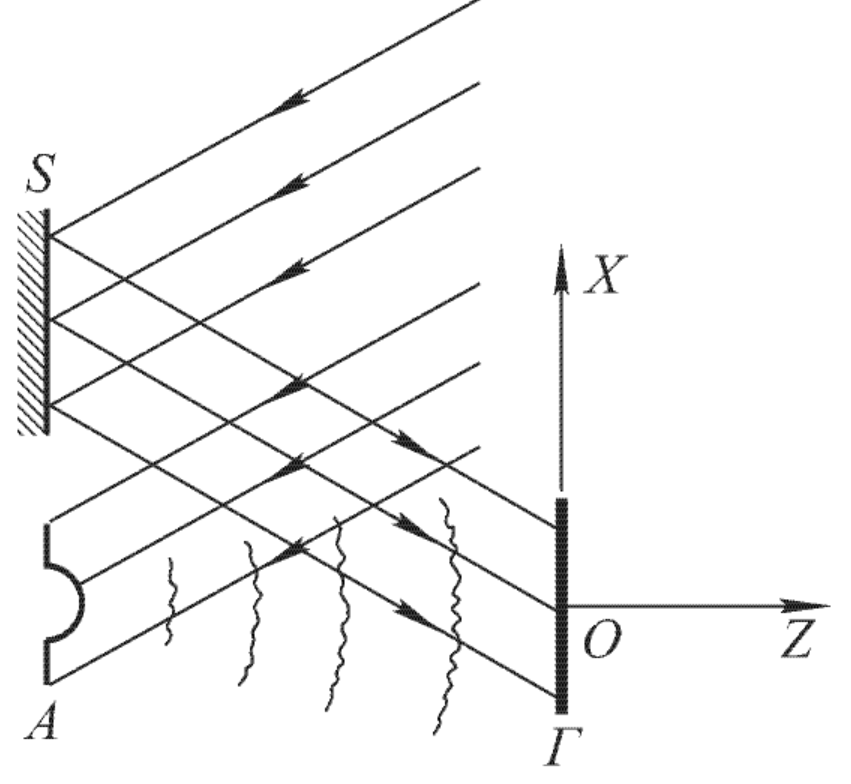
\includegraphics[width=0.28\textwidth]{figures/s54_1.png}
  \end{center}
\end{wrapfigure}
Идея голографии Габора заключается в том, что свет, попадая на объект рассеивается, и рассеянные лучи несут все информацию о форме и рельефе объекта. Однако для восстановления из таких лучей изображения нужна ещё информация о фазе изначально падавшего пучка, которую можно получить, если предварительно разделить этот пучок и часть его пустить на зеркало, чтобы переотразить в область, где мы хотим получать голограмму.
Пучок, рассеивающийся на предмете называется, называется \textit{предметным}, а несущий информацию о фазе -- \textit{опорным}.
Полученная картина на $\Gamma$ записывается, например на чувтсвительную пластину,  и называется голограммой, от греческого <<голог>> -- полный, <<графе>> -- пишу. Позже осветив её той же опорной волной можно получить восстановленное изображение объекта.

Запись голограммы -- очень тонкое дело. Необходимая степень монохроматичности света:
	$\boxed{\frac{\lambda}{\delta l} \gtrsim m}$,
	где $m$ -- максимальный порядок интерференции наблюдающийся при голографировнии.

Для хорошей установки и объекта с линейными размерами $L $ этот порядок можно оценить $\boxed{m \sim \frac{L}{\lambda}}$.
Таким образом должно быть: $\boxed{\delta\lambda < \frac{\lambda^2}{L}}$.

Требования к размеру источника тоже достаточно жестки: $\Delta x = \lambda/\alpha$, где $\alpha$ -- угол схождения крайних интерферирующих лучей. По порядку это что-то вроде $\alpha = h/l$, где $h$ -- ширина опорного пучка, а $l$ -- расстояния между предметом и голограммой. Таким образом $\boxed{\Delta x < \frac{\lambda l}{h}}$.

И так, о чем же сама голография. Представим поле рассеянной волны и отраженной:
\begin{equation*}
	u = a (\vc{r}) e^{i [\omega t - \Phi(\smallvc{r})]},
	\hspace{0.5 cm}
	v = b e^{i (\omega t - \smallvc{k} \smallvc{r})}.
\end{equation*}
Тут мы сделали упрощение, что поля не векторные, а скалярные, что для нас не сильно критично, и при таком упрощении $a(\vc{r})$, $\Phi(\vc{r})$ и $b$ будем считать вещественными. На пластинке $\Gamma$ интенсивность:
\begin{equation*}
	I  = v^* u + v u^* + v^* v + u^* u,
	\hspace{0.5 cm}
	I_0 = b a (x,y,0) e^{i[k_x x - \Phi(x,y,0)]} + b a (x,y,0) e^{-i[k_x x - \Phi(x,y,0)]} + b^2 + a^2(x,y,0).
\end{equation*}
где мы направили ось $Z$ перпендикулярно плоскости $\Gamma = XY$.

Допустим теперь, что нашу пластину, покрытую фотоэмульсией мы проявили и \href{https://youtu.be/y-MyaUcMkhs?t=252}{скопировали}, получив позитив голограммы. Пусть у позитива пропускаемость $D = I_0$, такую позитивную голограмму можно использовать для восстановления $u(\vc{r},t)$.
Для этого голограмму просвечивают таким же $v(\vc{r},t)$, он испытает дифракцию на голограмме типа как на диф-решетке. По методу Рэлея получим поле на выходе и будем искать решение волнового уравнения:
\begin{equation*}
	E_{\text{вых}} = D v (x,y,0) = I_{0} b e^{i (\omega t - k_x x)},
	\hspace{1 cm}
	\frac{\partial^2 E}{\partial x^2} + \frac{\partial^2 E}{\partial y^2} + \frac{\partial^2 E}{\partial z^2} + k^2 E = 0.
\end{equation*}
Будем искать решение для $E$ в виде $E = E_1 + E_2 + E_3 + E_4$, с граничными условиями:
\begin{equation*}
	\begin{aligned}
		&E_{1 \text{ вых}} = b^2 a(x,y,0) e^{i [\omega t - \Phi(x,y,0)]},\\
		&E_{2 \text{ вых}} = b^2 a(x,y,0) e^{i [\omega t + \Phi(x,y,0) - 2 k_x x]},	
	\end{aligned}
	\hspace{1 cm}
	\begin{aligned}
		&E_{3 \text{ вых}} = b^3 e^{i (\omega t - k_x x)},\\
		&E_{4 \text{ вых}} = b a^2(x,y,0) e^{i (\omega t - k_x x)}.
	\end{aligned}
\end{equation*}
Будем решать. Проще всего найти функцию $E_3 = b^3 e^{i (\omega t - \smallvc{k} \smallvc{r})} = b^2 v(\vc{r},t)$, это есть ни что иное, как опорная волна, распространяющаяся за голограмму.

Основной же интерес для голографии представляет собой поле $E_1$, $b$ -- постоянно, тогда:
\begin{equation*}
	E_1 = b^2 a (x,y,z) e^{i [\omega t - \Phi(x,y,z)]} = b^2 u (\vc{r},t).
\end{equation*}
Действительно, видим, что это волна, уходящая от голограммы. Она даст мнимое изображение объекта, в том же самом месте, в котором он находился до получения голограммы. 

Для нахождения $E_2$ сначала посмотрим на случай, когда опорный луч падает нормально плоскости голограммы, тогда $k_x = 0$, и немного другое граничное условие дадут решение
\begin{equation*}
	E_{2 \text{ вых}} = b^2 a(x,y,0) e^{i[\omega t + \Phi(x,y,0)]}
	\hspace{1 cm}
	\Rightarrow
	\hspace{1 cm}
	\tilde{E}_2 (x,y,z) = b^2 a (x,y,z) e^{i [\omega t + \Phi(x,y,z)]}.
\end{equation*}
Такая волна снова создаёт мнимое изображение, как и только что рассмотренная выше $E_1$, но она распространяется к голограмме, а не от нее, значит не может служить решением рассматриваемой нами задачи.
Чтобы починиться в уравнении Гельмгольца заменим $z \mapsto -z$
\begin{equation*}
	\frac{\partial^2 E}{\partial x^2} + \frac{\partial^2 E}{\partial y^2} + \frac{\partial^2 E}{\partial (-z)^2} + k^2 E = 0
	\hspace{1 cm}
	\Rightarrow
	\hspace{1 cm}
	E_2 = b^2 a(x,y,-z) e^{i[\omega t + \Phi(x,y,-z)]}.
\end{equation*}
Теперь волна идёт от голограммы, является решением нашей краевой задачи, и формирует таким образом действительное изображение.
Отвлечемся теперь от изложения материала из Сивухина, и обратимся к специализированной литературе в поисках чего-нибудь большего.
Вообще, можно дочитать этот 54 параграф, где Сивухин текстом описывает свойства и объемных голограмм тоже, можно открыт Кириченко, где это ещё снабжено и формулами. 
Здесь же я обращусь к дополнительной литературе из задавальника:\textit{Р. Кольер, Оптическая голография. – М. : Мир, 1973}.

Какие главы и параграфы взять для нашей программы.
\section{Кристаллооптика}

Поведение света всё также описывается уравнениями Максвелла
\begin{equation*}
    \rot \vc{H} = \frac{1}{c} \dot{\vc{D}},
    \hspace{5 mm} 
    \rot E = - \frac{1}{c} \dot{\vc{H}},
\end{equation*}
однако усложняются материальные уравнения:
\begin{equation*}
    D^j = \varepsilon_i^j E^i,
\end{equation*}
где $\varepsilon_{ij}$ -- \textit{тензор диэлектрической проницаемости}, или \textit{диэлектрический тензор}.
% Такая анизотропия приводит к неколлинеарности $\vc{D}$ и $\vc{E}$.

Рассмотрим плоские монохроматические волны вида
\begin{equation*}
    \vc{A} = \vc{A}_0 e^{i(\omega t - \smallvc{k} \cdot \smallvc{r})}, 
\end{equation*}
где $\vc{A} \in \{\vc{E},\, \vc{H},\, \vc{D}\}$. Понятно, что
\begin{equation*}
    \rot \vc{H} = -i \left[\vc{k} \times  \vc{H}\right],
    \hspace{5 mm} 
    \partial_t \vc{D} = - i \omega \vc{D}, \hspace{5 mm} \ldots
\end{equation*}
Подставив это в уравнения Максвелла, вводя верно волновой нормали $\vc{N} = \frac{v}{\omega} \vc{k}$, получаем
\begin{equation*}
    \vc{D} = - \frac{c}{v} \left[\vc{N} \times \vc{H}\right],
    \hspace{5 mm} 
    \vc{H} = \frac{c}{v} \left[\vc{N} \times \vc{E}\right],
\end{equation*}
где $v$ -- нормальная скорость волны. 

Актуально, как никогда, значение вектора Пойтинга
\begin{equation*}
    \vc{S} = \frac{c}{4\pi}\left[\vc{E} \times \vc{H}\right].
\end{equation*}

\begin{to_lem}
    Вектор пойтинга $\vc{S}$ определяет направление световых лучей, то есть $S \parallel \vc{u} = d_{\smallvc{k}} \omega$.
\end{to_lem}

Стоит заметит, что в кристаллая $\vc{S}$ и $\vc{N}$ не совпадают по направлению. 
Однако, как видно из формул, плоские волны в кристалле поперечн в отношении векторов $\vc{D}$ и $\vc{H}$. Вектора $\vc{E},\, \vc{D},\, \vc{N},\,  \vc{S}$ лежат в плоскости, перпендикулярной к вектору $\vc{H}$. 

Получается, что если $\vc{E}$ и $\vc{D}$ не сонаправлены, то зная направление $\vc{E}$ мы знаем направление и $\vc{D}$, а тогда и $\vc{H}$, и $\vc{N}$, $\vc{S}$ соответственно тоже. 
При $\vc{E} \parallel \vc{D}$ любая прямая $\bot \vc{E}$ может служить направлением магнитного поля. 
Подставляя $\vc{H}$ в $\vc{D}$ можем найти
\begin{equation*}
    \vc{D} = \frac{c^2}{v^2} \vc{E} - \frac{c^2}{v^2} \left(\vc{N} \cdot \vc{e} \right) \vc{N},
\end{equation*}
и, т.к. $(\vc{D} \cdot \vc{N})=0$, то скалярно умножая на $\vc{D}$ находим
\begin{equation*}
    v^2 = c^2 \frac{(\vc{D} \cdot \vc{E})}{D^2}.
\end{equation*}
Таким образом вектор $\vc{E}$ в кристале является \textit{главным}.

\subsection{Оптически одноосные кристаллы}

\begin{to_def}
    \textit{Оптически одноосными} называют кристаллы, свойства которых обладают симметрей вращения относительно некоторого направления, называемого \textit{оптической осью кристалла}.
\end{to_def}

Разложим $\vc{E}$ и $\vc{D}$ на составляющие параллельные оптической оси, и нормальный к ней, тогда
\begin{equation*}
    \vc{D}_\parallel = \varepsilon_\parallel \vc{E}_\parallel,
    \hspace{5 mm} 
    \vc{D}_\bot = \varepsilon_\bot \vc{E}_\bot,
\end{equation*}
где $\varepsilon_\parallel$ и $\varepsilon_\bot$ -- продольная и поперечные диэлектрические проницаемости кристалла. Плоскости, в которой лежат оптическая ось кристалла и нормаль $\vc{N}$, называется \textit{главным сечением кристалла}. 


\begin{to_def}
    Если электрический вектор $\vc{D}$ перпендикулярен к главному сечению, то скорость волны не зависит от направдения её распространения, такая волна называется \textit{обыкновенной}.
\end{to_def}

Тогда $\vc{D} \equiv \vc{D}_\bot$, тогда и $\vc{D} = \varepsilon_\bot \bar{E}$, соответственно 
\begin{equation*}
    \vc{D} = \varepsilon_\bot \vc{E},
    \hspace{0.5cm} \Rightarrow \hspace{0.5cm}
    \left.\begin{aligned}
        D &= H \textstyle \frac{c}{v} \\
        H &= E \textstyle \frac{c}{v}
    \end{aligned}\right.
    \hspace{5 mm} \Rightarrow \hspace{5 mm} 
    v = v_\bot \equiv \sub{v}{o} = \frac{c}{\sqrt{\varepsilon_\bot}}.
\end{equation*}

\begin{to_def}
    Если электрический вектор $\vc{D}$ лежит в главном сечении, то скорость волны зависит от направления распространенияЮ и такую волну называют \textit{необыкновенной}.
\end{to_def}

Вектор $\vc{E}$ в таком случае также лежит в главном сечении, и $\vc{E} = \vc{e}_N + \vc{E}_D$. В таком случае, верно
\begin{equation*}
    \vc{H} = \frac{c}{v} \left[\vc{N} \times \vc{E}_D\right],
    \hspace{5 mm} 
    E_D = \frac{\vc{E} \cdot \vc{D}}{D} = \frac{E_\parallel D_\parallel + E_\bot D_\bot}{D} = \frac{1}{D} \left(
        \frac{D_\parallel^2}{\varepsilon_\parallel} + \frac{D_\bot^2}{\varepsilon_\bot}.
    \right)
\end{equation*}
Соответсвующие проекции можно заменить на $D \sin \alpha$, где $\alpha$ -- угол между оптической осью и волновой нормалью. Вводя $\frac{1}{\varepsilon} = \frac{N^2_\bot}{\varepsilon_\parallel}+\frac{N^2_\parallel}{\varepsilon_\bot}$ можем перейти к
\begin{equation*}
    E_D = D\left(
        \frac{\sin^2 \alpha}{\varepsilon_\parallel} + \frac{\cos^2 \alpha}{\varepsilon_\bot}
    \right) = \frac{D}{\varepsilon},
    \hspace{5 mm} 
    H = \frac{c}{v} E_D,
    \hspace{0.5cm} \Rightarrow \hspace{0.5cm}
     v = \frac{c}{\sqrt{\varepsilon}} = c \sqrt{\frac{N^2_\bot}{\varepsilon_\parallel}+\frac{N_\parallel^2}{\varepsilon_\bot}}\equiv v_\parallel.
\end{equation*}


Когда $N_\bot =0$, то понятно, что $v = c/\sqrt{\varepsilon_\bot} = v_\bot = \sub{v}{o}$, -- нет разницы между обыкновенной и необыкновенной. В случае $N_\parallel = 0$  верно, что $v = \sub{v}{e} \overset{\mathrm{def}}{=} c/\sqrt{\varepsilon_\parallel}$. 

Термин оптическая ось введен для обозначения прямой, вдоль которой обе волны распростаняются с одинаковыми скоростями, и таким прямых в общем случае, поэтому кристалл называется \textit{оптически двуосным}. В рассмотренном частном случае оси совпали, и получился \textit{оптически одноосный} кристалл.


\begin{to_lem}
    В общем случае волна, вступающая в кристалл изотропной среды, разделяется внутри кристалла на две линейно поляризованные волны: обыкновенную, вектор электрической индукции которой перпендикулярен к главному сечению,
    и необыкновенную с вектором электрической индукции, лежащим в главном сечении.
\end{to_lem}

\textbf{Про показатели преломления}. В кристаллая верны законы преломления для \textit{волновых нормалей}: их направления подчиняются закону Снеллиуса
\begin{equation*}
    \frac{\sin \varphi}{\sin \psi_\bot} = n_\bot,
    \hspace{5 mm} 
    \frac{\sin \varphi}{\sin \psi_{\parallel}} = n_{\parallel},
\end{equation*}
где $n_\bot$ и $n_\parallel$ -- показатели прелоления обыкновенной и необыкноуенной волн, т.е.
\begin{equation*}
    n_\bot = \frac{c}{v_\bot} = \sub{n}{o},
    \hspace{5 mm} 
    n_\parallel = \frac{c}{v_\parallel} = \left(\frac{N^2_\bot}{\varepsilon_\parallel}+\frac{N^2_\parallel}{\varepsilon_\bot}\right)^{-1/2}.
\end{equation*}
Постоянная $\sub{n}{o}$ называется \textit{обыкновенным показателем преломления}. Когда необыкновенная волна распространяется перпендикулярно к оптической оси $(N_\bot=1)$, 
\begin{equation*}
    n_\parallel = \sqrt{\varepsilon_\parallel} \overset{\mathrm{def}}{=} \sub{n}{e}.
\end{equation*}
Величина $\sub{n}{e}$ -- \textit{необыкновенный показатель преломления кристалла}. 


\textbf{Двойное лучепреломление}. При преломлении на первой поверхности пластинки волна внутри кристалла разделяется на обыкноыенную, и необыкновенную. Эти волны поляризованы во взаимно перпендикулярных плоскостях и распространяются внутри пластинки в разных направлниях и с разными скоростями. Таким образом можно добиться пространственного разделения двух лучей. 
% рис 1



\textbf{Поляризационные устройства}. Комбинация кристаллов -- поляризационная призма\footnote{
    Самая первая призма -- \textit{николь}, 1828 г.
} . Существуют \textit{однолучевые} (на полном внутренне отражении) и \textit{двулучевые}. 

\begin{to_def}
    Допустимая разность углов наклона между крайними лучами падающего на призму пучка называется \textit{апертурой полной поляризации призмы}.
\end{to_def}

\begin{to_def}
    \textit{Дихроизм} -- свойство кристаллов, состоящее в различном поглощении веществом света в зависимости от его поляризации. Всего различают: \textit{линейный дихроизм} (при $\bot$ направлениях линейной поляризации); \textit{эллиптический дихроизм} (различное поглощение для правой и левой эллиптической поляризации); \textit{круговой дихроизм} (различные направления круговой поляризации, иначе -- \textit{эффект Коттона}). 
\end{to_def}






\textbf{Анализ поляризованного света}. \textit{Пластинка в четверть волны} ($\lambda/4$), вносит дополнительную разность фаз в $\pi/2$ между проходящими через неё лучами, поляризованными во взаимно перпедикулярных плоскостях. 

 %-


\textbf{Интерференция поляризованных лучей}.


% посыл на будущее -- интерактивная среда, -- вставки, по возможности, сценариев из математики и питона.




 %-


\textbf{Волны в двуосных кристаллах}.

 %-

\textbf{Лучи и волновые нормали.}

 %-





\subsection{Двойное преломление в электрическом и магнитном полях (эффект Керра)}

\textit{Электрический эффект Керра состоит в том}, \textit{что многие изотропные тела при введении в постоянное электрическое поле становится оптически анизотропным}. В частности, ведут себч как одноосные двупреломляющие кристаллы, оптическая ось которых параллельна приложенному электрическому полю. 


Пусть внешнее поле $\vc{E}_0$ \textit{однородно}. Понятно, что $\sub{n}{e}-\sub{n}{o}$ зависит от $\vc{E}_0$ в виде
\begin{equation*}
    \sub{n}{e} - \sub{n}{o} = q E_0^2,
\end{equation*}
для малых полей, где $q$ зависит только от вещества и от $\lambda$. В таком случае разность фаз между обыкновенной и необыкновенными лучами будет
\begin{equation*}
    \varphi = \frac{2\pi}{\lambda}(\sub{n}{e} - \sub{n}{o}) l = 2 \pi B l E^2,
\end{equation*}
где $l$ -- толщина образца, а $B \equiv q/\lambda$ -- \textit{постоянная Керра}. \textbf{Явление Керра объясняется анизотропией самих молекул.} 

Для эффекта Керра в газах, в случае полностью анизотропных молекул, можно показать, что при $\vc{E} \parallel \vc{E}_0$ показатель преломления будет \textit{необыкновенным}, тогда
\begin{equation*}
    n = 1 + \frac{2\pi}{3} N \beta,
\end{equation*}
где $\beta$ -- поляризуемость молекулы вдоль оси молекулы. Если же $\vc{E} \bot \vc{E}_0$, то  показатель преломления будет обыкновенным, и
\begin{equation*}
    \sub{n}{o} = 1 + 2 \pi N \beta \langle \sin^ \vartheta \rangle,
\end{equation*}
где $\vartheta$ -- угол\footnote{
    \red{Дописать}.
}  между $\vc{E}$ и $\vc{s}$.

Забавный факт: из полученных соотноешний можем получить
\begin{equation*}
    \frac{\sub{n}{e}-n}{\sub{n}{o}-n} = -2,
\end{equation*}
что выполняется для большинства веществ. 


Проводя некоторый аккуратны расчёт можем получить выражение для постоянной Керра:
\begin{equation*}
    \sub{n}{e} - \sub{n}{o} = \frac{n-1}{5} \frac{\beta}{kT} E_0^2.
\end{equation*}




Рассмотрим \textit{ангармонический осциллятор}  при наличии внешнего постоянного электрического поля $E_0$ 
\begin{equation*}
    \ddot{r} + 2 \gamma \dot{r} + \omega_0^2 r + \beta r^2 = -\frac{e}{m}E_0,
\end{equation*}
где $\beta$ -- постоянная. Считая $r = r_0 + q$ можем перейти к уравнению с новой частотой
\begin{equation*}
    \ddot{q} + 2 \gamma \dot{q} + (\omega_0^2+ 2\beta r_0) q =0,
\end{equation*}
откужа видно изменение частоты колебания на 
\begin{equation*}
    \Delta \omega_0^2 = -\frac{2 e \beta}{m \omega_0^2} E_0^2.
\end{equation*}
Смещение собственных частот меняет кривую дисперсии, т.е. показатель преломления $n$ среды. В простейшем случае, когда $\omega_0$ одна (см. \S 84), изменение $n$ определяется выражением
\begin{equation*}
    \Delta n = \frac{\partial n}{\partial \omega_0^2} \Delta \omega_0^2 = - \frac{\partial n}{\partial \omega_0^2} 
    - \frac{\partial n}{\partial \omega_0^2} \frac{2e\beta}{m \omega_0^2} E_0 = 
    \frac{\partial n}{\partial \omega} \frac{e\beta}{m \omega \omega_0^2} E_0.
\end{equation*}
При фиксированном внешнем $\vc{E}_0$ величина $\Delta n$ зависит от направления распространения света.
Это сказывается на двойном преломлении среды. \textit{Изменеие двойного преломления вещества из-за смещения собственной частоты во внешнем электрическом поле называется электрооптическим эффектом Поккельса}.

В этом эффекте изменения пропорциональны первой степени $E_0$. \textit{Эффект Поккельса может наблюдаться только в 
кристаллах, не обладающих центром симметрии.} Устройство, основанное на эффекте Поккельса, называют \textit{ячейкой Поккельса}. 

Она представляет собой кристалл, помещаемый между двумя скрещенными николями. 
Такое устройство действует так же, как и ячейка Керра. Николи
не пропускают свет, когда нет внешнего электрического поля,
но при наложении такого поля пропускание появляется. 
Необходимо, чтобы кристалл до наложения внешнего электрического
поля не давал двойного преломления. Этого можно достигнуть,
если взять оптически одноосный кристалл, вырезанный 
перпендикулярно к оптической оси, а свет направить вдоль этой оси.
Внешнее поле Eq может быть направлено либо перпендикулярно
(поперечный модулятор света), либо параллельно 
распространению света (продольный модулятор).





\subsection{Вращение плоскости поляризации}


Если линейно поляризованный свет проходит через плоскопараллельный слой вещества, то в некоторых случаях плоскость поляризации света оказывается повернутой относительно своего исходного положения. Это явление называется \textit{вращением плоскости поляризации} или оптической активностью. Если вещество не находится во внешнем магнитном поле, то оптическая активность и вращение плоскости поляризации называются \textit{естестыенными}. В противоположнос случае говорят о \textit{магнитном вращении плоскости поляризации}, или \textit{эффекте Фарадея}. 


Вращение против часовов -- \textit{положительное}, по часовой -- \textit{отрицательное}. Это свойство, как и в случе с шурупом, не зависит от того, в каком из двух прямо противоположных напралний распространяетя свет\footnote{
    Если свет заставить пройти туда и обратно через естественно-активное вещество, отразив его от
    зеркала, то плоскость поляризации возвратится к своему исходисходному направлению.
} . 


В области прозрачности и малого поглощения эта история хорошо согласуется с опытом формула Друде
\begin{equation*}
    \xi = \alpha L,
    \hspace{5 mm} 
    \alpha = \sum_i \frac{B_i}{\lambda^2-\lambda_i^2},
\end{equation*}
где $B_i$ -- постоянные, $\lambda_i$ -- длины волн, соответсвующие собтсвенным чатсота рассматриваемого вещества. 



По Френелю вращение плоскости поляризации -- проявление \textit{кругового двойного лучепрпеломления}. Две волны, которые могут распространятся в оптически активной среде с разными скоростями, поляризованы \textit{по кругу}: по левому и по правому.

Покажем достаточность такого предположения:
\begin{equation*}
    \left.\begin{aligned}
        E_x &= A \cos \xi \cos (\omega t - k z), \\
        E_y &= A \sin \xi \cos (\omega y - k z),
    \end{aligned}\right.
    \hspace{5 mm} 
    \xi = - \alpha z,
    \hspace{0.5cm} \Rightarrow \hspace{0.5cm}
    \left.\begin{aligned}
        E_x &= \textstyle \frac{A}{2} \cos(\omega t - k z + \alpha z) + \textstyle \frac{A}{2} \cos(\omega t - k z - \alpha z), \\
        E_y &= \textstyle \frac{A}{2} \cos(\omega t - k z + \alpha z + \pi/2) + \textstyle \frac{A}{2} \cos(\omega t - kz - \alpha z - \pi/2).
    \end{aligned}\right.
\end{equation*}
Разложим полученную волну на две: $\vc{E} = \sub{\vc{E}}{п} + \sub{\vc{E}}{л}$, где для  $ \sub{\vc{E}}{п}$ и $\sub{\vc{E}}{л}$ имеет смысл ввеси $\sub{k}{п} = k-\alpha$  и $\sub{k}{л} = k + \alpha$. Полученные волны соответствуют правой и левой круговой поляризации. Скорости этих волн определяются выражениями
\begin{equation*}
    \sub{v}{п} = \frac{\omega}{k-\alpha}, \hspace{5 mm} \sub{v}{л} = \frac{\omega}{k+\alpha},
\end{equation*}
и соответсвующие покзатели преломления $n = c/v$. Подробнее,
\begin{equation*}
    \sub{n}{r} = \frac{c}{\sub{v}{r}} = \frac{c}{\omega}(k-\alpha),
    \hspace{5 mm} 
    \sub{n}{l} = \frac{c}{\sub{v}{l}} = \frac{c}{\omega}(k+\alpha),
    \hspace{0.5cm} \Rightarrow \hspace{0.5cm}
    \alpha = \frac{\omega}{2c}(\sub{n}{l}-\sub{n}{r}).
\end{equation*}




Френель выдвинул гипотезу, что возможно независимое распространения поляризованных по кругу волн, с сохранением поляризации, которую подтвердил эксперементально. Тем самым задача объяснения вращения плоскости поляризации была сведена к задаче объяснения кругового двойного лучепреломления.

Поляризованные по кругу в противоположных направлениях
волны в окрестности полос или линий поглощения могут 
отличаться не только скоростями распространения, но и 
коэффициентами поглощения. Тогда они выйдут с различными 
амплитудами. Если падающий свет был поляризован линейно, то 
выходящий будет поляризован эллиптически. Это явление 
называется круговым дихроизмом. 
Опыты Фарадея показали, что при наличии внешнего магнитного поля вдоль оптической оси системы, угол поворота зависит от длины пути $l$ и напряженноести внешнего поля $B$, как
\begin{equation*}
    \xi = R\, l B,
\end{equation*}
де $R$ -- \textit{постоянная Верде}, или \textit{магнитная вращательная способность}. 

При внесении в магнитное поле $\vc{B}$ у осцилляторов вещества появляются две новые резонансные частоты $\omega_0 + \Omega$ и $\omega_0 - \Omega$, где $\Omega$ -- ларморовская частота. Эти собственны частоты проявляеются не только в испускании (\textit{прямой эффект Зеемана}), но и в поглощении света (\textit{обратный эффект Зеемана}). 

Нормальные волны, которые могут распространятся вдоль магнитного поля, поляризованы по кругу. Когда направления распространения света и магнитного поля совпадают, большей частоте $\omega_+ = \omega_0 + \Omega$ соответсвует вращение по, а меньшей $\omega_-$ -- против часовой стрелки, если смотреть в направлении магнитного поля. Так как $\omega_+$ и $\omega_-$ различны, то происходит сдвиг фаз волн, а соответсвенно, и повород плоскости поляризации на гол
\begin{equation*}
    \xi = \frac{\omega l}{2c} (n_- - n_+) = \frac{\pi l}{\lambda} (n_- - n_+).
\end{equation*}

Если построить $n_- - n_+$, то можно увидеть, что, как и в случае ларморовского вращения $\Omega$, вращение плоскости поляризации определяется только направлением магнитного поля $\vc{B}$ и не зависят от направления распространения света.  При изменение на противоположное направления распространеняи света не изменятся, в противоположность естественного вращения. 

Вообще, в эффекте Фарадея, воспользовавшись формулой Зеемана можно получить \textit{формулу Беккереля} для постоянной Верде:
\begin{equation*}
    R = - \frac{e}{2 mc^2} \lambda \frac{d n}{d \lambda},
\end{equation*}
где $m$ -- масса электрона, $e > 0$ -- его абсолютный заряд.  


Ещё можно было бы поговорить про \textit{эффект Макалюзо и Корбино}, объясненный Фохтом, но оставим это на светлое будущее. 






\section{Нелинейная оптика}



\subsection{Нелинейная поляризацим среды}

% § 91, 99, 100).

При распространении света в среде нелинейные явления в оптике связаны прежде всего с \textit{нелинейной зависимостью} вектора поляризации среды $\vc{P}$ от напряженности электрического поля $\vc{E}$ световой волны. Если поле $\vc{E}$ ещё не <<очень сильное>>, то вектор $\vc{P}$ можно разложить во степеням $\vc{E}$:
\begin{equation*}
    P_j = \alpha_{jk} E_k + \alpha_{jkl} E_k E_l + \alpha_{jklm} E_k E_l E_m + \ldots, 
\end{equation*}
где $\alpha_{jk}$ -- \textit{линейная поляризуемость среды}, а тензоры высших порядков называют соответственно квадратичной, кубичной, и т.д. \textit{поляризуемостями}. Поле $\vc{E}$ предполагаем монохроматичным, среду однороднойЮ немагнитной, без дисперсии, а $\alpha$ -- функции частот $\omega$. Для изотропной среды все тензоры $\alpha$ вырождаются в скаляры. 



% Про нелинейные эффекты: познакомимся с выпрямление света, генерациоей второй гармоники и самофокусировка света. 
В средах, в которых все точки явяются центрами симметрии, квадратичный член равен нулю. Однако, можем рассмотреть \textit{качественно} процессы, полагая
\begin{equation*}
    \vc{P} = \alpha \vc{E} + \alpha_2 E \vc{E} + \alpha_3 E^2 \vc{E} + \ldots,
\end{equation*}
где мы принимаем ущербность такого приближения, но зато можем сделать несколько правильных шагов. Разобьем поляризацию, а также индукцию, на линейную и нелиненую: $\vc{P} = \sub{\vc{P}}{l}+\vc{P}_{\textnormal{nl}}$, где нелинейная часть $\sub{\vc{P}}{nl} = \alpha_2 E \vc{E} + \alpha_3 E^2 \vc{E} + \ldots$, а линейная $\sub{\vc{P}}{l} = \alpha \vc{E}$. Тогда и $\vc{D} = \vc{E} + 4 \pi \vc{P}$ предсавится, как $\sub{\vc{D}}{\vc{l}=E}+4 \pi \sub{\vc{P}}{l}$ и нелинейная $\sub{\vc{D}}{nl}=4 \pi \vc{P}_{\textnormal{nl}}$. Линейная часть $\sub{\vc{D}}{l}=\varepsilon \vc{E}$, где $\varepsilon$ -- диэлектрическая проницаемость. Теперь можем записать уравнения Максвелла в виде
\begin{equation*}
\left.\begin{aligned}
    \rot \vc{H} &= \frac{1}{c} \frac{\partial \vc{D}}{\partial t}, \\
    \rot \vc{E} &= - \frac{1}{c} \frac{\partial \vc{H}}{\partial c}, \\
    \div \vc{D} &= 0, \\
    \div \vc{H} &= 0, \\
\end{aligned}\right.
\hspace{0.75cm} \Rightarrow \hspace{0.75cm}
\left.\begin{aligned}
            \rot \vc{H}  &=  \frac{\varepsilon}{c} \frac{\partial \vc{E}}{\partial t} + \frac{4 \pi}{c} \frac{\partial \sub{\vc{P}}{nl}}{\partial t} , \\
    \rot \vc{E}  &=  \frac{1}{c} \frac{\partial \vc{H}}{\partial t}, \\
    \div(\varepsilon \vc{E}) &= - 4\pi \div \sub{\vc{P}}{nl}, \\
    \div \vc{H} &= 0.
    \end{aligned}\right.    
\end{equation*}
Система решается \textit{методом последовательных приближений}. В нулевом приближение $\sub{\vc{P}}{nl}=0$, получаются уравнения \textit{линейной электродинамики}. В качестве нулевого приближения рассмотрим
\begin{equation*}
    \vc{E} = \vc{E}_0 = \vc{A} \cos(\omega t - \vc{k} \cdot \vc{r}),
\end{equation*}
где $\vc{k}^2 = \varepsilon \omega^2/c^2$. Для нахождения первого приближения вместо $\vc{E}$ подставим $\vc{E}_0$, после чего снова получим линейные уравнения, но неоднородные. Правые части могут восприниматься как если бы каждый $\d V$ переизлучал волны аки \textit{диполь Герца} с моментом $\sub{\vc{P}}{nl} \d V$. Такими итерациями может найти сколь угодно приближений. 


Вообще среда диспергирует. Формально всё будет работать если взять эту охапку диффуров и решать её оидельно для слагаемых с частотой $\omega$, частотой $2\omega$, и т.д., подставляя везде свои $\varepsilon$. По идее это работает. 
\subsection{Первое приближение. Генерация вторых гармоник.}

В нулевом приближении можем найти нелинейную добавку
\begin{equation*}
    \sub{P}{nl} = \alpha_2 E_0^2 = \frac{\alpha_2 A^2}{2} + \frac{\alpha_2 A^2}{2} \cos\left[2(\omega t - \vc{k} \cdot \vc{r})\right].
\end{equation*}
Как ни странно -- это вполне адекватный результат, первое слагаемое называют \textit{оптическим детектированием}, илиоптическим выпрямлением, -- возникновением в нелинейной среде постоянной электрической поляризации при прохождении мощной световой волны. 

Второе слагаемое гармонически меняется во времени. Оно вызывает \textit{генерацию второй гармоники в нелинейной среде}, т.е. волны с частотой $\omega_2 = 2 \omega$. Найдём поле этой гармоники:
\begin{equation*}
    \left.\begin{aligned}
        \rot \vc{H} &= \frac{\varepsilon[2\omega]}{c} \frac{\partial \vc{E}}{\partial t} + i \omega \frac{4 \pi \alpha_2}{c} A \vc{A} e^{2 (i \omega t - \smallvc{k} \smallvc{r})}, \\
        \rot \vc{E} &= \frac{1}{c}\frac{\partial \vc{H}}{\partial t}, \\
        \div \vc{E} &= \div \vc{H} = 0,
    \end{aligned}\right.
    \hspace{0.5cm} \Rightarrow \hspace{0.5cm}
    \vc{E} = A_1 e^{2 i (\omega t - \smallvc{k} \smallvc{r})},
    \hspace{5 mm} 
    \vc{H} = B_1 e^{2 i (\omega t - \smallvc{k} \smallvc{r})},
\end{equation*}
что соответсвует частному решению от вынужденных колебаний. Из второго уравнения следует, что $\vc{E} \bot \vc{H}$, также верно, что $(\vc{k} \cdot \vc{A}_1) = (\vc{k} \cdot \bar{B}_1)=0$, т.е плоская волна поперечна относительно $\vc{E}$ и $\vc{H}$. Учитывая, что $k^2 c^2 = \omega^2 \varepsilon[\omega]$ можем получить:
\begin{equation*}
    \vc{A}_1 = \frac{2 \pi \alpha_2}{\varepsilon[\omega]-\varepsilon[2\omega]} A \vc{A}.
\end{equation*}
Если же к частном решению, добавим общее, то увидем, что можем подобрать такую его амплитуду, чтобы интенсивность второй гармоники в начале координат обращалась в нуль:
\begin{equation*}
    \vc{E}_1 = \frac{2 \pi \alpha_2}{\varepsilon[\omega]-\varepsilon[2\omega]} A \vc{A} \left(
        \cos[2(\omega t - \vc{k} \cdot \vc{r})] - \cos[2 \omega t - \vc{k}_2 \cdot \vc{r}]
    \right),
\end{equation*}
где $k_2^2 = \omega_2^2 \varepsilon[2\omega]/c^2$. Возводя в квадрат и усредняя можем найти интенсивность
\begin{equation*}
    I_1 \sim \frac{\alpha_2^2 \omega^2 x^2 I^2}{n^2 c^2} \left(\frac{\sin \beta}{\beta}\right)^2,
    \hspace{5 mm} 
    \beta = \frac{(2\vc{k} - \vc{k}_2)\cdot \vc{r} }{2} = \frac{(2k-k_2)x}{2},
\end{equation*}
где $x$ -- пройденное расстояние. Тут принебрегли различием $n[\omega]$ и $n[2\omega]$. 


Таким образом с возрастанием $x$ возрастает интенсивность второй гармоники, когда $\beta \in [0, \pi/2]\cup[\pi, 3\pi/2]$, и т.д. В этих сдучаях \textit{энергия переходит от исходной волны ко второй гармоники}. На других интервалах энергия возвращается от второй, к первой. Условие $\beta=\pi/2$ определяет расстояние, до которого происходит перекачка энергии. Это расстояние называется \textit{когерентной длиной}, для которого верно, что
\begin{equation*}
    \sub{L}{coh} = \frac{\lambda}{4|n[\omega]-n[2\omega]},
\end{equation*}
где $\lambda$ -- длина исходной волны. 

Когда $n[\omega]=n[2\omega]$ верно, что $2 \vc{k} = \vc{k}_2$, тогда и $\sub{L}{coh}$ обращается в бесконечность. Это условие -- \textit{фазовый синхронизм}. 


Ещё в 1962 году было эксперментально продемонстрирована возможность осущиствить фазовый синхронизм на частотах $\omega$ и $2 \omega$ между обыкновенной и необыкновенной волной в некоторых кристаллах. 


Аналогичное явление -- \textit{генерация волн с суммарной и разностной частотами}. Если на нелинейную среду направить два можных пучка света с различными частотами $\omega_1$ и $\omega_2$, то из неё будет выходить свет с частотами $\{\omega_1,\, \omega_2,\, 2 \omega_1,\, 2 \omega_2,\, \omega_1+\omega_2,\, \omega_1-\omega_2\}$. Так можно получить излучение в инфракрасной и ультрафиолетовой области, например, $\approx 80$ нм. 
\subsection{Второе приближение. Самофокусировка.}



Для нахождения \textit{второго приближения} воспользуемся 
\begin{equation*}
    \sub{\vc{P}}{нл} = \alpha_2 (E_0 + E_1)(\vc{E}_0 + \vc{E}_1) + \alpha_3 E_0^2 \vc{E}_0,
\end{equation*}
однако учитывая только изотропные среды переходим к $\alpha_2 = 0$, а тогда
\begin{equation*}
    \sub{\vc{P}}{nl} = \frac{3 \alpha_3 A^2}{4} \vc{A} \cos\left[\omega t - \vc{k} \vc{r}\right] + 
    \frac{\alpha_3 A^2}{4} \vc{A} \cos[3\left(\omega t - \vc{k} \vc{r}\right)],
\end{equation*}
где второе слагаемое соответствует генерации тритьей гармоники.


Интересно  взглянуть на первое слагаемое: множитель $\vc{A} \cos[\omega t - \vc{k} \vc{r}]$ -- исходная падающая волна $\vc{E}_0$, которую можно заменить на $\vc{E}$, тогда
\begin{equation*}
    \rot \vc{H} - \frac{1}{c}\left[
        \varepsilon(\omega) + 3 \pi \alpha_3 (\omega) A^2
    \right] \partial_t \vc{E} = 0,
    \hspace{0.5cm} \Rightarrow \hspace{0.5cm}
    n = n_0 + n_2 A^2,
\end{equation*}
где учет рассматриваемого слагаемого эквивалентен изменению $\varepsilon(\omega)$ среды.



Вообще есть другие причины такого поведения: свет вообще давит на среду, греет среду, что приводит к изменению плотности и показателя преломления среды. В жидкостях это может быть высокочастотный эффект Керра, но во всех этих случаях $\Delta n \sim A^2$. К слову, $n_2$ бывает $>0$ и $<0$.


Так приходим к прохождению пучка через оптических неоднородную среду, в которой луч загибается в сторону большего показателя преломления. С этим связано явление \textit{самофокусировки} ($n_2 > 0$) и дефокусировки $(n_2 < 0)$.



Рассмотрим плоскопараллельный пучок лучей кругового сечения, диаметра $D$. Показатель преломления в пространстве с пучком $n = n_0 + n_2 A^2$, пусть $n_2 > 0$. Из-за дифракции пучок расширяется, однако все направления луче сосредоточатся в пределах конса с углом при вершине $2 \sub{\vartheta}{диф}$, где $\sub{\vartheta}{диф} = 1.22 \lambda/(D n_0)$. Предельный угол скольжения $\vartheta_0$ определяется соотношением
\begin{equation*}
    \cos \vartheta_0 = \frac{n_0}{n_0 + n_2 A^2},
    \hspace{0.5cm} \Rightarrow \hspace{0.5cm}
    \vartheta_0^2 \approx 2 A^2 \frac{n_2}{n_0}.
\end{equation*}
Еслм $\sub{\vartheta}{диф} > \vartheta_0$ то пучок будет расширяться. При $\sub{\vartheta}{диф} > \vartheta_0$ пучок начнём сжиматься в тонкий шнур, -- \textit{самофокусировка}. 


При $\sub{\vartheta}{диф} = \vartheta_0$ имеет место \textit{самоканализация}, для которой можем найти необходимую мощность пучка
\begin{equation*}
    P = \frac{c n_0 A^2}{8 \pi} \frac{\pi D^2}{4} = \frac{c n_0 D^2}{32} A^2,
    \hspace{0.5cm} \Rightarrow \hspace{0.5cm}
    \sub{P}{порог} \approx c \frac{(0.61\, \lambda)^2}{16 n_2}.
\end{equation*}
Расстояние от края среды, на которой фокусируются крайние лучи пучка, легко оценить:
\begin{equation*}
    \sub{f}{эф} = \frac{D}{2 \sub{\vartheta}{диф}} \approx \frac{n_0 D^2}{2.44\, \lambda},
\end{equation*}
что называют \textit{эффективным фокусным расстоянием для крайних лучей пучка}. 



\sbs{13}{Порядок убывания коэффициентов Фурье абсолютно непрерывных функций}


\begin{to_lem}
    Если производная $f^{(k-1)}$ абсолютно непрерывна и производные до $k$-й включительно\footnote{
        Для $k$-й достаточно существования почти всюду.
    }  находятся в $L_1 (\mathbb{R})$, то
    \begin{equation*}
        c_f (y) = \int_{-\infty}^{+\infty} f(x) e^{-ixy} \d x = o \left(\frac{1}{y^k}\right),
        \hspace{5 mm}
        y \to \infty.
    \end{equation*}
    \label{lem8d43}
\end{to_lem}


\begin{uproof}
    Всё как раньше, но слагаемые вижа $f^{(l)} (x) e^{-ixy} |_{-\infty}^{+\infty}$ исчезают в силу конечности пределов $f^{(l)}$ на бесконечности. Так как $f^{(l+1)} \in L_1 (\mathbb{R})$, то $f^{(l)}$ имеет конечные пределы в $-\infty$ и $+\infty$, которые должны быть равны нулю, так как $f^{(l)}$ конечного интеграла.
    % \red{Я бы и эту штуку посмотрел в другой книжке.}
\end{uproof}

\section{Световоды}


\subsection{Введение}


\begin{to_def}
    \textit{Оптический волновод} -- диэлектрическая структура, по которой может распространяться электромагнитная энергия в видимой и инфракрасной областях спектра. 
\end{to_def}

Можно выделить ступенчатый и градиентный профиль волновода (рис. \ref{waveguide}).
\begin{figure}[ht]
    \centering
    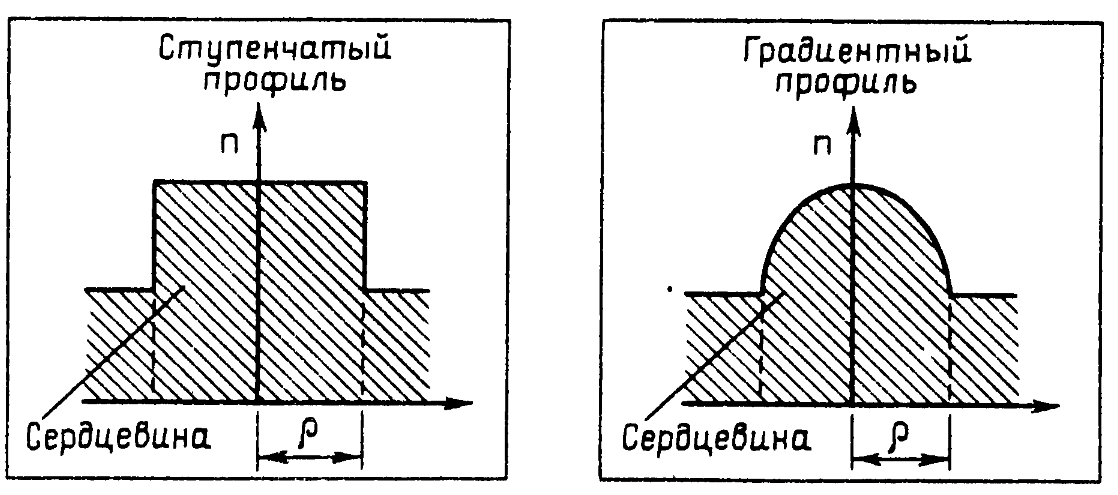
\includegraphics[height=0.17\textwidth]{figures/13_1.png}
    \hspace{5 mm} 
    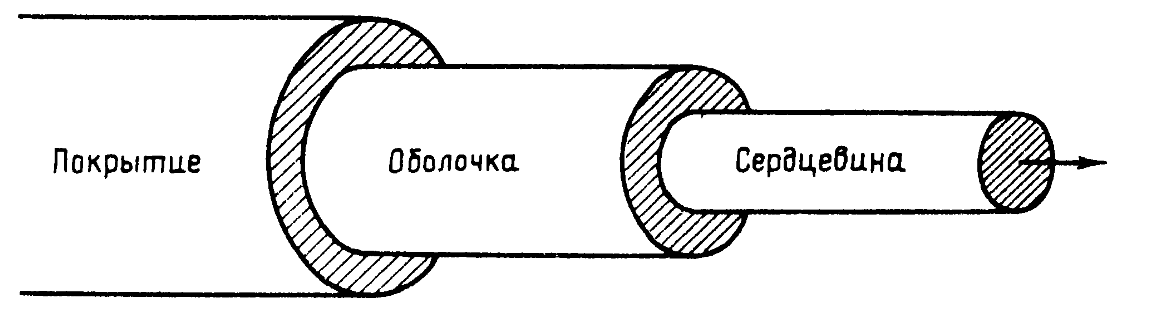
\includegraphics[height=0.12\textwidth]{figures/13_2.png}
    \caption{Профиль показателя преломления для типичных оптических волокон.}
    \label{waveguide}
\end{figure}
Обычно покрытие оказывается полностью изолировано от сердцевины, так что его влиянем можно пренебречь. 


\textbf{Многомодовые и одномодовые волноводы}. Оптические волноводы можно условно разделить на две группы -- \textit{многомодовые} (большая сердцевина) и \textit{одномодовые} (маленькая сердцевина). Для многомодовых световодов справедлво условие
\begin{equation*}
    \frac{2\pi \rho}{\lambda} \sqrt{\sub{n}{co}^2 - \sub{n}{cl}^2} \gg 1,
\end{equation*}
где $\rho$ -- характерный размер сердцевины, $\lambda$ -- длина волны света в свободном пространстве, $\sub{n}{co}$ -- максимальное значение показателя преломления сердцевины, а $\sub{n}{cl}$ -- показатель преломления оболочки. 
% см. часть I
%  часть II -- одномодовые

\textbf{Лучевой подход}. Показатель преломления обычно слабо меняется на масштабах $\lambda$ (по крайней мере для многомодовых), таким образом адекватно описывать происходящее в терминах лучей. 
В таком\footnote{
    Альтернативный подход к описанию распространения света в многомодовых волноводах -- коротковолновое приближение для ЭМ волн. 
}  случае \textit{пренебрегается всеми волновыми эффектами}. 
% см. гл. 6-9, локальные плоские волны


Важно, что в линиях связи большой протяженности случается уширение распространяющихся импульсов. В случе идеальных многомодовых волоконных световодов уширение вполне описывается геом-оптикой. 


\subsection{Направляемые лучи в планарных волноводах}

Классический многомодовый волновод характеризуется значениями $\sub{n}{cl}$ и $\sub{n}{co}$, а также толщиной сердцевины $2 \rho$, что вместе с длиной волны может быть собрано в один безразмерный параметр
\begin{equation*}
    V = \frac{2\pi}{\lambda} \rho \sqrt{\sub{n}{co}^2 - \sub{n}{cl}^2},
\end{equation*}
собственно лучевой подход применим только  при $V \gg 1$. 


В случае ступенчатого профиля всегда можем описать $n(x)$ как
\begin{equation*}
    n(x) = \left\{\begin{aligned}
        &\sub{n}{co}, &-\rho < x < \rho; \\
        &\sub{n}{cl}, &|x| \geq \rho,
    \end{aligned}\right.
\end{equation*}
что может упроситить работу с построением лучей. Одна и наиболее важных задач -- определение условий, при которых луч является \textit{направляемым}, т.е. распространяется вдоль непоглащающего волновода без потерь мощности. 






\subsection{Типы волн}

В общем случае в волоконном световоде могут существовать три типа волн: \textit{направляемые}, \textit{вытекающие} и \textit{излучаемые}. 



 см. страницу 37.
\subsection{Рэлеевское рассеяние}


 см. страницу 100-104

\subsection{Изгибы}


см 153 - 156
\subsection{Дисперсия}


Можно посмотреть \href{http://foos.sfedu.ru/glava2/2.2.html}{здесь}.

Вообще на странице 186. Нулевая на с. 297. 














\section{Ряд Фурье в пространстве \texorpdfstring{$L_2$}{L2}}
% \sbsnum{1}{Возмущенное движение}
% что-то

\sbsnum{2}{Основные теоремы прямого метода Ляпунова}

% \subsubsection*{Теорема Ляпунова об устойчивости движения}


Здесь и далее для простоты рассматриваем установившееся движение.

\begin{to_thr}[Теорема Ляпунова об устойчивости]
    Если дифференциальные уравнения возмущенного движения таковы, что существует знакоопределенная функция $V$, производная которой $\dot{V}$ в силу этих уравнений является знакопостоянной функцией противоположного знака с $V$, или тождественно равной нулю, то \red{невозмущенное движение} устойчиво.
\end{to_thr}










\begin{to_thr}[Теорема Ляпунова об асимптотической устойчивости]
    Если дифференциальные уравнения возмущенного движения таковы, что существует знакоопределенная функция $V(x_1, x_2, \ldots, x_m)$, производная которой $\dot{V}$ в силу этих уравнений есть знакоопределенная функция противоположного знака с $V$, то невозмущенное движение асимптотически устойчиво.
\end{to_thr}



\subsubsection*{Теоремы о неустойчивости}

\begin{to_def}
    Окрестностью положения равновесия, считая, что положение равновесия находится в точке $q^1=\ldots=q^n=0$, назовём область такую, что
    \begin{equation*}
        |q^i| < h, \hspace{1 cm} (i=1, 2,\ldots,m).
    \end{equation*}
\end{to_def}

\begin{to_def}
    Областью $V > 0$ назовём какую-либо область окрестности положения равновесия, в которой $V(x_1, x_2, \ldots, x_m) > 0$. Поверхность $V = 0$ назовём границей области $V >0$.
\end{to_def}

\begin{to_thr}[Теорема Читаева о неустойчивости]
    Если дифференциальные уравнения возмущенного движения таковы, что существует функция $V(x_1, \ldots, x_m)$ такая, что в сколь угодно малой окрестности положения равновесия существует область $V > 0$ и во всех точках области $V > 0$ производная $\dot{V}$ в силу уравнений принимает положительные значения, \textbf{то} невозмущенное движение неустойчиво.
\end{to_thr}

\begin{to_def}
    Функцию $V$, удовлетворяющую теореме Читаева о неустойчивости, называют \textit{функцией} \textit{Читаева}.
\end{to_def}



\begin{to_thr}[I теорема Ляпунова о неустойчивости движения]
    Если дифференциальные уравнения возмущенного движения таковы, что существует функция $V(x_1, \ldots, x_m)$ такая, что ее производная $\dot{V}$ в силу этих уравнений есть функция знакоопределенная, сама функция $V$ не является знакопостоянной, противоположного с $\dot{V}$ знака, то невозмущенное движенние неустойчиво.
\end{to_thr}

\begin{to_thr}[II теорема Ляпунова о неустойчивости движения]
    Если дифференциальные уравнения возмущенного движения таковы, что существует функция $V$ такая, что её производная, в силу этих уравнений, в области положения равновесия может быть представлена в виде
    \begin{equation*}
        \dot{V} = \textnormal{\ae} V + W,
    \end{equation*}
    где \textnormal{\ae} -- положтельная постоянная, а $W$ \textbf{или} тождественно обращается в нуль, \textbf{или} представляет собой знакопостоянную функцию. Если $W$ -- знакопостоянная функция, а $V$ \textbf{не является}  знакопостоянной функцией: $W V < 0$, \textbf{то} невозмущенное движение неустойчиво (ну и если $w \equiv 0$).
\end{to_thr}




\sbsnum{4}{Влиянение диссипативных и гироскопических сил на устойчивость равновесия консервативной системы}



\begin{to_thr}[Теорема Томсона-Тэта-Четаева]
    Если в некотором изолированном положении равновесия потенциальная энергия имеет строгий локальный минимум, то при добавлении гироскопических и диссипативных сил с полной диссипацией это положение равновесия становится асимптотически устойчивым.
\end{to_thr}
















\subsubsection*{Влияние гироскопических и диссипативных сил на
неустойчивое равновесие}

Разложим до квадратичных членов кинетическую и потенциальную энергию системы, и приведем к каноническому виду
\begin{equation*}
    T = \frac{1}{2}\sum_{i=1}^n \dot{\theta}_i^2,
    \hspace{1 cm}
    \Pi = \frac{1}{2} \sum_{i=1}^{n} \lambda_i \theta_i^2.
\end{equation*}
Если $\Pi$ положительно определена, то все величины $\lambda_i$ положительны, и положение устойчиво. Если же присутствуют отрицательные $\lambda_i$, то положение равновесия неустойчиво (\red{по теореме о неустойчивости по первому приближению}). 

\begin{to_def}
    Величины $\lambda_i$ Пуанкаре предложил называть \textit{коэффициентами устойчивости}. Число отрицательных коэффициентов устойчивости называется \textit{степенью неустойчивости}. 
\end{to_def}


\begin{to_thr}[]
    \textbf{Если} среди коэффициентов устойчивости хотя бы один является отрицательным, \textbf{то} изолированное положение равновесия не может быть стабилизировано диссипативными силами с полной диссипацией.
\end{to_thr}

\begin{to_thr}[]
    \textbf{Если} степень неустойчивости изолированного положения равновесия консервативной системы нечетна, \textbf{то} стабилизация его добавлением гироскопических сил невозможна. \textbf{Если} степень неустойчивости четна, \textbf{то} гироскопическая стабилизация возможна.
\end{to_thr}

\begin{to_thr}[]
    \textbf{Если} изолированное положение равновесия консервативной системы имеет отличную от нуля степень неустойчивости, \textbf{то} оно остается неустойчивым при добавлении гироскопических сил и диссипативных сил с полной диссипацией.
\end{to_thr}

\begin{to_def}
    Устойчивость, существующую при одних потенциальных силах, называют \textit{вековой}, а устойчивость, полученную с помощью гироскопических сил, -- \textit{временной}.
\end{to_def} 
\sbs{16}{Неравенство Бесселя и оптимальность коэффициентов Фурье}


\begin{to_thr}[Оптимальность коэффициентов Фурье]
    Для всякой $f \in L_2[-\pi, \pi]$ и данного числа $n$ лучшее по норме $L_2$ приближение $f$ тригонометрическим многочленом $\sum_{-n}^{+n} c_k e^{ikx}$ дают коэффициенты Фурье
    \begin{equation*}
        c_k = \frac{1}{2\pi} \int_{-\pi}^{\pi} f(x) e^{ikx} \d x.
    \end{equation*}
\end{to_thr}

\begin{uproof}
    Воспользуемся скалярным произведением в $L_2$, занумеруем $e^{ikx}$ в некотором порядке $\varphi_1$, $\varphi_2$, $\ldots$, где далее будет важна лишь орогональность этих функций относительно введенного скалярного произведения. Пусть мы приближаем $\varphi = \sum_{k=1}^N a_k \varphi_k$ и оптимизируем $a_k$, тогда
    \begin{equation*}
        \left\|
            f - \sum_{k=1}^{N} a_k \varphi_k
        \right\|_2^2 = \|f\|_2^2 - 
        \sum_{k=1}^{N} \bar{a}_k (f, \varphi_k) - \sum_{k=1}^{N} a_k (\varphi_k, f) + \sum_{k=1}^{N} |a_k|^2 \|\varphi_k\|_2^2.
    \end{equation*}
    Далее, по определению коэффициентов Фурье в виде $(f, \varphi_k) = c_k \|\varphi\|_2^2$ находим
    \begin{equation*}
        \left\|
            f - \sum_{k=1}^{N} a_k \varphi_k
        \right\|_2^2 = \|f\|_2^2 - \sum_{k=1}^{N} \left(
            \bar{a}_k c_k + a_k \bar{c}_k - |a_k|^2
        \right) \|\varphi_k\|_2^2 = 
        \|f\|_2^2 - \sum_{k=1}^{N} |c_k|^2 \|\varphi_k\|_2^2 + \sum_{k=1}^{N} |c_k - a_k|^2 \|\varphi_k\|_2^2,
    \end{equation*}
    откуда оптимально положить $a_k = c_k$. 
\end{uproof}


\begin{to_lem}[неравенство Бесселя]
    Из доказательства предыдущей теоремы, можем получить, что
    \begin{equation*}
        \left\|f - \sum_{k=1}^N c_k \varphi_k \right\|_2^2 = 
        \|f\|_2^2 - \sum_{k=1}^{N} |c_k|^2 \|\varphi_k\|_2^2,
        \hspace{0.7 cm} \Rightarrow \hspace{0.7   cm}
        \|f\|_2^2 \geq  \sum_{k=1}^{N} |c_k|^2 \|\varphi_k\|^2_2,
        \hspace{0.5cm} \overset{\mathrm{trig}}{\Rightarrow}  \hspace{0.5cm}
        \|f\|_2^2 \geq 2\pi \sum_{k=-n}^n |c_k|^2.
    \end{equation*}
    % \red{Точно ли до $n$?}
\end{to_lem}

\begin{to_lem}[Представление действительнозначной функции]
    Для действительнозначной функции представление в виде ряда Фурье перепишется в виде
    \begin{equation*}
        f = a_0 + \sum_{k=1}^{n} (a_k \cos kx + b_k \sin kx),
        \hspace{0.25 cm}
        a_0 = \frac{1}{2\pi} \int_{-\pi}^{+\pi} f(x) \d x,
        \hspace{2.5 mm} 
        a_k = \frac{1}{\pi}\int_{-\pi}^{\pi} f(x) \cos kx \d x,
        \hspace{0.25 cm}
        b_k = \frac{1}{\pi} \int_{-\pi}^{\pi} f(x) \sin kx \d x,
    \end{equation*}
    для $k \geq 1$. Неравенство Бесселя тогда запишется так:
    \begin{equation*}
        \|f\|_2^2 \geq \frac{\pi}{2} |a_0|^2 + 
        \pi \sum_{k=1}^{\infty} (|a_k|^2 + |b_k|^2).
    \end{equation*}
\end{to_lem}

 
\sbs{17}{Полные системы в пространстве \texorpdfstring{$L_2$}{L2}} 


Пусть $\{\varphi_i\}$ -- ортогональная система в $L_2$. Допустим $f = \sum_i c_i \varphi_i$, где коэффиценты $c_i$ могут быть найдены непосредственно:
\begin{equation*}
    c_i = \frac{(f,\, \varphi_i)}{\left(\varphi_i,\, \varphi_i\right)},
\end{equation*}
что упрощается в случае ортонормированной системы до $c_i = (f,\, \tilde{\varphi}_i)$. Числа $c_i$ и называются \textit{коэффицентами Фурье элемента} $f$ в ортогональной системе $\varphi_i$. 


В таких терминах можем определить и \textit{ряд Фурье} элемента $f$ по ортогональной системе $\{\varphi_k\}$:
\begin{equation*}
    f \sim \sum_{k=1}^{\infty} \frac{(f,\, \varphi_i)}{\left(\varphi_i,\, \varphi_i\right)} \varphi_k,
\end{equation*}
где если система $\varphi_k$ конечна, то ряд сводится к конечной сумме. 

Так например можно выделить ортогональную систему $\{1, \cos k x, \sin kx; \ k \in \mathbb{N}\}$. Или, например, многочлены Лежандра
\begin{equation*}
    P_n (x) = \frac{1}{2^n n!} \frac{d^n}{d z^n} \left(z^2-1\right)^n,
\end{equation*}
образующих ортогональную систему. 

 
\begin{to_def}
    Система $\{\varphi_\alpha; \alpha \in \mathcal A\}$ векторов нормированного пространства $X$ называется \textit{полной по отношению к множеству} $E \subseteq X$ (полной в $E$), если любой вектор $x \in E$ можно сколь угодно точно в смысле нормы пространства $X$ приблизить конечными линейными комбинациями векторов системы. Другими словами $E \subset \bar{L}\{\varphi_\alpha\}$ -- замыкание линейной оболочки векторов. 
\end{to_def}



\begin{to_thr}[условие полноты ортогональной системы]
    Пусть $X$ -- линейное пространство со скалярным произведением, а $\varphi_k$ -- конечная или счётная система ортогональных векторов в $X$. Тогда следующие условия эквивалентны: 
    \vspace{-2mm}
    \begin{enumerate*}
        \item система $\{\varphi_k\}$ полна по отношению к множеству $E \subseteq X$;
        \item для любого вектора в $f \in E \subset X$ имеет место разложение в ряд Фурье в смысле нормы;
        \item для любого вектора $f \in E \subset X$ имеет место равенство Парсеваля $\|f\|^2 = \sum_k |(f, \varphi_k)|^2/(\varphi_k, \varphi_k)$.
    \end{enumerate*}
\end{to_thr}

\begin{uproof}
Из (1) $\Rightarrow$ (2) в силу экстремального свойства коэффициентов Фурье. Из (2) в (3) по теореме Пифагора. Из (3) $\Rightarrow$ (1) т.к. ввиду леммы о перпендикуляре по теореме Пифагора ...
\red{по Зоричу можно дописать}.
\end{uproof}



\begin{to_def}
    Система элементов линейного нормированного простанства $X$ называется \textit{базисом пространства} $X$, если любая конечная её подсистема состоит из линейно независимых векторов и любой вектор $x \in X$ может быть представлен в виде $f = \sum_k \alpha_k x_k$, где $\alpha_k$ -- коэффициенты из поля констант пространства $X$, а сходимость понимается по норме пространства $X$. 
\end{to_def}






Для доказательства неравенства Бесселя достаточно требовать ортогональность системы. В случае же равенства Парсеваля необходима \textit{полнота} системы -- возможность приблизить любую функцию $L_2$ линейной комбинацикй функций рассматриваемой системы сколь угодно точно. 



 
\sbs{18}{Равенство Парсеваля для Фурье функций из \texorpdfstring{$L_2[-\pi, \pi]$}{L2[-pi, pi]}} 



\begin{to_thr}[Сходимость ряда Фурье в среднеквадратичном]
    Для вской комплекснозначной $f \in L_2 [-\pi, \pi]$
    \begin{equation*}
        f = \sum_{k=-\infty}^{\infty} 
        c_k e^{ikx} = 
        \lim_{n \to \infty} \sum_{k=-n}^{n} c_k e^{ikx},
        \hspace{10 mm} 
        c_k = \frac{1}{2\pi} \int_{-\pi}^{+\pi} f(x) e^{ikx} \d x
    \end{equation*}
    в смысле сходимости суммы в пространстве $L_2[-\pi, \pi]$, а также выполняется равенство Парсеваля
    \begin{equation*}
        \|f\|_2^2 = 2 \pi \sum_{k=-\infty}^{\infty} |c_k|^2.
    \end{equation*}
\end{to_thr}

\begin{uproof}
    Сначала функцию $f$ приближаем по $L_2$ норме тригонометрическим многочленом. Формула для квадрата точности приближения
    \begin{equation*}
         \left\|
            f - \sum_{k=1}^{N} c_k \varphi_k
         \right\|_2^2 = \|f\|_2^2 - 2\pi \sum_{k=1}^{N} |c_k|^2 < \varepsilon,
     \end{equation*} 
     откуда при $N \uparrow$ можем говорить про сходимость ряда Фурье по $L_2$ норме по определению. Также получаем в пределе в неравенстве Бесселя равенство Парсеваля. 
\end{uproof}

Стоит заметить что в последней теореме использовали <<симметричное>> сумирование -- \textit{суммирование в смысле главного значения}:
\begin{equation*}
    v.p. \ \sum_{k=-\infty}^{+\infty} c_k e^{ikx}  = \lim_{n \to \infty} \sum_{k=-n}^{n}  c_k e^{ikx}.
\end{equation*}

\texttt{Пока мы не доказали, что в полученную формулу можно подставить хоть одно конкретное значение $x$. Тот факт, что ряд Фурье функции из
$L_2[-\pi, \pi]$ на самом деле сходится к этой функции почти всюду, был доказан Л. Карлесоном (1966), а до этого был известен как гипотеза Лузина.} 

 


\section{Тригонометрический ряд Фурье и его сходимость}
\sbs{19}{Интегральное представление частичных сумм ряда Фурье, ядро Дирихле}

\begin{to_def}
    Обозначим \textit{частичную сумму} тригонометрического ряда Фурье для $2\pi$-периодической функции $f$ как
    \begin{equation*}
        T_n (f, x) = \sum_{k=-n}^n c_k (f) e^{ikx}.
    \end{equation*}
\end{to_def}

\begin{to_lem}
    Для $n$-й частичной суммы ряда Фурье $2\pi$-периодической функции имеет место формула в виде свёртки
    \begin{equation*}
        T_n (f, x) = \int_{-\pi}^{\pi} f(x+t) D_n (t) \d T,
    \end{equation*}
    с ядром Дирихле
    \begin{equation*}
        D_n (t) = \frac{1}{2\pi} \frac{\sin \big(\left(n+\frac{1}{2}\right) t\big)}{\sin\left(\frac{1}{2} t\right)}.
    \end{equation*}
\end{to_lem}

\begin{uproof}
    По определению:
    \begin{equation*}
        T_n[f](x) = \sum_{k=-n}^{n} c_k e^{ikx}
        =
        \frac{1}{2\pi} \sum_{k=-n}^{n} \int_{-\pi}^{+\pi}
        f(\xi) e^{ikx-ik\xi} \d \xi
        = \bigg/
            \xi = x + t
        \bigg/ = \int_{-\pi}^{+\pi} f(x+t) \left(
            \frac{1}{2\pi} \sum_{k=-n}^{n} e^{-ikt}
        \right) \d t.
    \end{equation*}
    Теперь раскрываем геометрическую прогрессию:
    \begin{equation*}
        D_n (t) = \frac{1}{2\pi} \sum_{k=-n}^{n} e^{-itk} = 
        - \frac{e^{int}}{2\pi} \frac{e^{it}-e^{-2int}}{1 - e^{it}} = 
        \frac{e^{i(n+1/2)t}-e^{-i(n+1/2)t}}{2\pi \left(e^{it/2}-e^{-it/2}\right)} = 
        \frac{1}{2\pi} \frac{\sin(n+1/2)t}{\sin t/2}.
    \end{equation*}
\end{uproof}


\begin{to_lem}[Равномерная ограниченность интегралов от ядра Дирихле]
    Существует такая константа $C$, что 
    \begin{equation*}
        \left|
        \int_a^b D_n (t) \d t
        \right| \leq C
    \end{equation*}
    для любых $a, b \in [-\pi, \pi], \ n \in \mathbb{N}$.
\end{to_lem}


\begin{uproof}
    Заметим, что $t/\sin(t/2)$ -- положительная и ограниченная на $[-\pi, \pi]$ функция, тогда вынесем её из под знака интеграла:
    \begin{equation*}
        \bigg| \int_{a}^{b} \frac{1}{2\pi} \frac{\sin \big(\left(n+\frac{1}{2}\right) t\big)}{\sin\left(\frac{1}{2} t\right)} \d t \bigg| \sim
        \bigg|
           \int_a^b \frac{\sin \big(\left(n+\frac{1}{2}\right) t\big)}{t} \d t 
        \bigg| \sim 
        \bigg|
            \int_{a'}^{b'}  \frac{\sin t}{t} \d t
        \bigg|.
    \end{equation*}
    А оставшееся выражение принимает значения $\in [-1, 1]$, так что имеет конечный интеграл на отрезке и ограничен на всей числовой прямой.
\end{uproof}

Также можем оценить интеграл от ядра Дирихле:
\begin{equation*}
    D_n (t) = \frac{1}{2\pi} \sum_{k=-n}^{n} e^{-ikt},
    \hspace{0.5cm} \Rightarrow \hspace{0.5cm}
    \int_{-\pi}^{\pi} D_n (t) = 1,
    \hspace{0.5cm} \Rightarrow \hspace{0.5cm}
    T_n[f](x) - f(x) = \int_{-\pi}^{+\pi} \left(
        f(x+t) -f(x)
    \right) D_n(t) \d t,
\end{equation*}
что исследуется равномерным принципом локализации. 
\sbs{20}{Принцип локализации для рядов Фурье и равномерный принцип локализации}


\begin{to_thr}[принцип локализации]
    Если $f$ -- $2\pi$-периодическая абсолютно интегрируемая функция, то существование и значение предела последовательности её частичных сум Фурье $T_n[f](x)$ в любой точке $x_0 \in \mathbb{R}$ зависит только от существования и значения предела при $n \to \infty$ интеграла
    \begin{equation*}
        \frac{1}{\pi} \int_0^\delta D_n(t) \left(
            f(x_0 + t) + f(x_0 - t)
        \right) \d t,
    \end{equation*}
    иначе говоря сходимость ряда Фурье в точке $x_0$ определяется лишь поведением функции $f$ в любой сколь угодно малой окрестности $x_0$. 
\end{to_thr}

\begin{uproof}
    Во-первых, по чётности ядра Дирихле, можем записать
    \begin{align*}
        T_n[f](x) &= \frac{1}{\pi} \int_{0}^{\pi} D_n(t) \left(
            f(x+t) + f(x-t)
        \right) \d t = 
        \left(
            \frac{1}{\pi} \int_{0}^{\delta}  + \frac{1}{\pi} \int_{\delta}^{\pi} 
        \right) D_n(t) \left(
            f(x+t) + f(x-t)
        \right) \d t.
    \end{align*}
    Подробнее рассмотрим последнее слагаемое:
    \begin{equation*}
        \frac{1}{\pi} \int_{\delta}^{\pi} \frac{f(x+t)+f(x-t)}{2 \sin (t/2)} \sin\left(
            \left(n + \textstyle\frac{1}{2}\right)t
        \right) \d t = o(1), \hspace{5 mm} n \to \infty,
    \end{equation*}
    так как $\frac{f(x+t) + f(x-t)}{2 \sin (t/2)}$ интегрируемое по интегрируемости $f$ и ограниченности $\frac{1}{\sin(t/2)}$. Оставшаяся велична стремится к $0$ по лемме Римана об осцилляции.
\end{uproof}


\begin{to_thr}[Равномерный принцип локализации]
    Запищем для $\delta \in (0, \pi)$
    \begin{equation*}
        T_n (f, x) - f(x) = 
        \int_{-\pi}^{\pi} 
        \left(
            f(x+t) - f(x)
        \right) D_n (t) \d t =
        \int_{-\delta}^{\delta} \left(
            f(x+t) - f(x)
        \right) D_n (t) \d t + 
        \int_M 
        (f(x+t)-f(x)) D_n (t) \d t,
    \end{equation*}
    где $M = \left\{t \mid \delta \leq |t| \leq \pi\right\}$. Если $f \in L_1 [-\pi, \pi]$, то
    \begin{equation*}
        \int_M \left(
            f(x+t) - f(x)
        \right) D_n (t) \d t
        \ \to \ 0, \hspace{0.5 cm} n \to \infty.
    \end{equation*}
    Если $f$ ограничена на отрезке $[a, b]$, то это выражение стремится к нулю равномерно по $x \in [a, b]$.
\end{to_thr}

\begin{uproof}
    Делаем то же, что и раньше, но подводим всё к лемме о равномерной осцилляции:
    \begin{equation*}
        \bigg| \int\limits_{a}^{b}  f(x+t) \sin\big(\left(n + \textstyle \frac{1}{2}\right) t \big) \d t \bigg| \sim 
        \bigg|
            \int\limits_{a}^{b} f(x+t) e^{i\left(n + \frac{1}{2}\right)t} \d t
        \bigg| = 
        \bigg|
            \int\limits_{x +a}^{x + b}  f(\xi) e^{\left(
                i\left[
                    n + \textstyle \frac{1}{2}
                \right] \xi - i \left[
                    n + \textstyle \frac{1}{2}
                \right] x
            \right)} \d \xi
        \bigg| = 
        \bigg|
            \int\limits_{x +a}^{x + b}  f(\xi) e^{\left(
                i\left[n + \textstyle \frac{1}{2}\right] \xi
            \right) }\d \xi
        \bigg|,
    \end{equation*}
    где уже можем применить лемму о равномерной осцилляции в силу $f \in L_1$. 
\end{uproof}

 
\sbs{21}{Признак Липшица равномерной сходимости ряда Фурье}

\begin{to_def}
    Функция $f$ называется гёльдеровой степени $\alpha > 0$, если для любых $x, \, y$ из области определения
    \begin{equation*}
        |f(x) -f(y)| \leq C |x-y|^{\alpha}
    \end{equation*}
    с некоторой константой $C$.
\end{to_def}


\begin{to_thr}[Признак Липшица сходимости ряда Фурье]
    Для абсолютно интегрируемой $2\pi$-периодической функции, которая является гёльдеровой с некоторыми $C$, $\alpha > 0$ на интервале $(A, B) \supset [a, b]$
    \begin{equation*}
        T_n (f, x) \to f(x)
    \end{equation*}
    равномерно по $x \in [a, b]$ при $n \to \infty$.
\end{to_thr}

\begin{uproof}
    Вспомним локальное представление $T_n[f](x) - f(x)$, как
    \begin{equation*}
        \bigg|
            \int_{-\delta}^{\delta} \left(f(x+t)-f(x)\right) D_n (t) \d t
        \bigg|  \leq 
        C \int_{-\delta}^{\delta} \frac{|t|^\alpha}{2\pi}
        \frac{1}{|\sin t/2|} \d t \leq 
        \frac{C}{2} \int_{-\delta}^{\delta} |t|^{\alpha-1} \d t \leq \frac{C}{\alpha} |\delta|^\alpha,
    \end{equation*}
    где мы воспользовались мыслью, что $\pi |\sin t/2| \geq t$ на $[-\pi, \pi]$. По произвольности $\delta$ и равномерного принципа локализации следует, что $T_n[f](x) - f(x)$ может быть равномерно сделано сколь угодно маленьким при некотором $\delta > 0$ и $n$. 
\end{uproof}


 
\sbs{22}{Признак Дирихле равномерной сходимости тригонометрического ряда Фурье на отрезке}

\begin{to_thr}[Признак Дирихле сходимости ряда Фурье]
    Для абсолютно интегрируемой $2\pi$-периодической функции, которая является непрерывной с ограниченной вариацией на интервале $(A, B) \supset [a, b]$
    \begin{equation*}
        T_n (f, x) \to f(x)
    \end{equation*}
    равномерно по $x \in [a, b]$ при $n \to \infty$.
\end{to_thr}


% \red{Далее несколько лемм, сформулированных в виде задач, а именно признак Дирихле сходимости ряда Фурье в точке, признак Липшица сходимости ряда Фурье в точке, признак Дини сходимости ряда Фурье в точке. Ага, это 13 тема. А потом будут темы 14 - 17.}



 
\sbs{23}{Признаки Липшица, Дирихле и Дини сходимости Фурье в точке}

\begin{to_thr}[признак Дини]
    Пусть $f$ -- $2\pi$-периодиечкая $\in L_1[-\pi, \pi]$. Если $x$ -- точка непрерывности или разрыва I рода и $\exists  \delta \in (0, \pi)$ такое, что $\int_0^\delta |f^*_x (t)|/t \d t$ сходится, то 
    ряд Фурье $f$ сходится в $x$ к $\frac{1}{2} \left(f(x+0)+ f(x-0)\right)$.
\end{to_thr}

Выше использовалась функция $f^*_x (t) = f(x-t) + f(x+t) - f(x-0) - f(x+0)$. В случае, если точка была регулярной, то Фурье к ней и сходится. Аналогично можно сформулировать это утвержение, как
\begin{equation*}
    \int_{-\delta}^{\delta} \bigg|\frac{f(x+t)-f(x)}{t} \bigg| \d t \text{ \ сходится}
    \hspace{0.5cm} \Rightarrow \hspace{0.5cm}  
    \text{ряд Фурье сходится к $f(x)$.}
\end{equation*}
Признаке Дирихле и Липшица в точке являются локальными аналогами признаков на отрезке. 





 
\sbs{24}{Почленное дифференцирование и интегрирование рядов Фурье}

\begin{to_thr}[Почленное интегрирование ряда Фурье]
    Пусть $f \in L_1 [-\pi, \pi]$ соответствует не обязательно сходящийся ряд Фурье, записанный в действительном виде как
    \begin{equation*}
        a_0 + \sum_{n=1}^{\infty} (a_n \cos nx + B_n \sin nx).
    \end{equation*}
    Тогда ряд Фурье можно почленно интегрировать, то есть выполняется формула
    \begin{equation*}
        \int_a^b f(x) \d x =    
        \frac{1}{2} a_0 (b-a) + 
        \sum_{n=1}^{\infty} \left(
            \frac{a_n \sin n x}{n} -
            \frac{b_n \cos nx }{n}
        \right) \bigg|_a^b.
    \end{equation*}
\end{to_thr}


 
\sbs{25}{Теорема Фейера}



\begin{to_def}
    Определим \textit{ядро Фейера} 
    \begin{equation*}
        \Phi_n (t) = 
        \frac{D_0 (t) + D_1 (t) + \ldots + D_n (t)}{n+1} = 
        \frac{1}{2\pi} \sum_{k=-n}^{n} 
        \frac{n+1 - |k|}{n+1} e^{ikx},
    \end{equation*}
    как усреднение ядер Дирихле. Соответствующая \textit{сумма Фейера} будет соответствовать усреднением первых $n+1$ частичных сумм ряда Фурье,
    \begin{equation*}
        S_n (f, x) = \int_{-\pi}^{\pi} 
        f(x+\xi) \Phi_n (\xi) \d \xi = 
        \frac{T_0 (f, x) + \ldots + T_n (f, x)}{n+1}.
    \end{equation*}
\end{to_def}

Записав
\begin{equation*}
    D_n (t) 
    =
    \frac{1}{2\pi}
     \frac{\sin \left( \left(n + \frac{1}{2}\right)t\right)}{\sin \left(\frac{1}{2} t\right)} 
     = 
     \frac{1}{4\pi}
    \frac{
    \cos nt - \cos \left((n+1)t\right)
    }{
    \sin^2 \left(\frac{1}{2}t\right)
    },
\end{equation*}
и суммируя, получаем
\begin{equation*}
    \Phi_n (t) = 
    \frac{1}{4 \pi}
    \frac{
        1 - \cos \left((n+1)t\right)
    }{
        (n+1) \sin^2 \left(\frac{1}{2}t\right)
    }
    =
    \frac{1}{2\pi}
    \frac{
        \sin^2 \left(
            \frac{n+1}{2}t
        \right)
    }{
        (n+1) \sin^2 \left(\frac{1}{2}t\right)
    }
\end{equation*}


\begin{to_thr}
    Для непрерывной $2\pi$-периодической $f$ 
    \begin{equation*}
        S_n (f, x) \rightrightarrows f(x),
    \end{equation*}
    то есть сходится равномерно.
\end{to_thr}
 
\sbs{26}{Представление котангенса и косеканса. Формула дополнения для бета-функции}

\begin{to_lem}
    \red{Разложим $\cos ax$ на отрезке $[-\pi, \pi]$ при $a \notin \mathbb{Z}$ в ряд Фурье.} Легко получить, что
    \begin{align*}
        \ctg x
        &=
        v. p. \sum_{k=-\infty}^{\infty} \frac{1}{x-\pi k} \\
        \frac{1}{\sin x}
        &=
         v. p. \sum_{k=-\infty}^{\infty} \frac{(-1)^k}{x-\pi k} \\
        \sin x
        &=
        x \prod_{k=1}^{\infty} \left(
            1 - \frac{x^2}{\pi^2 k^2}
        \right).
    \end{align*}
\end{to_lem}


\begin{to_lem}
    \textit{Формула дополнения} для бета-функции про $p \in (0, 1)$
    \begin{equation*}
        B(p, 1-p) = \int_0^1 t^{p-1} (1-t)^{-p} \d t = \frac{\pi}{\sin \pi p}.
    \end{equation*}
\end{to_lem}

\begin{to_lem}
    Для $0 < |x| < \pi$ верно, что
    \begin{equation*}
        \frac{1}{x} - \ctg x = 
        \sum_{n, k \geq 1} \frac{2 x^{2k-1}}{\pi^{2k} n^{2k}},
    \end{equation*}
    \red{
        откуда можно получить значения сумм $\sum_{n=1}^{\infty} \frac{1}{n^2}$ и $\sum_{n=1}^{\infty} \frac{1}{n^4}$.
    }
\end{to_lem}




\section{Интеграл Фурье и преобразование Фурье}
\sbs{27}{Интеграл Дирихле}


\begin{to_lem}[нормировка интеграла Дирихле]
    Выполняется
    \begin{equation*}
        v.p.\ \int_{-\infty}^{+\infty}  D_h(t) \d t = v.p. \ \int_{-\infty}^{+\infty}  \frac{\sin ht}{\pi t} = 1.
    \end{equation*}
\end{to_lem}

\begin{uproof}
Интеграл можем свести к условно сходящемуся интегралу
\begin{equation*}
    \int_{0}^{\infty}  \frac{\sin t}{t} \d t =\frac{\pi}{2}.
\end{equation*}
Рассмотрим интеграл с параметром $y \in [0, +\infty)$:
\begin{equation*}
    I(y) = \int_{0}^{\infty} e^{-yt} \frac{\sin t}{t} \d t,
\end{equation*}
который сходится абсолютно при $y > 0$. Разложим интеграл на два и проанализируем отдельно:
...
\end{uproof}




\sbs{28}{Представление функции интегралом Фурье, свёртка с ядром Дирихле для интеграла Фурье}



Представление функции \textit{интегралом Фурье} -- формула вида
\begin{equation*}
    f(x) \sim v.p.\ \int_{-\infty}^{+\infty}  c(y) e^{ixy} \d y,
\end{equation*}
где по аналогии с коэффициентами ряда Фурье
\begin{equation*}
    c(y) = \frac{1}{2\pi} \, v.p. \ \int_{-\infty}^{+\infty} f(x) e^{-ixy} \d x,
\end{equation*}
что будет сходиться  к определенным достаточно хорошим функциям.    


Введем также \textit{частичный интеграл Фурье}:
\begin{equation*}
    T_h (f, x) = \int_{-h}^{h} c(y) e^{ixy} \d y = \frac{1}{2\pi} \int_{-h}^{h} \left(
        v.p. \int_{-\infty}^{+\infty} f(\xi) e^{-(\xi-x)y} \d \xi
    \right) \d y.
\end{equation*}
Далее будем считать $f \in L_2 (\mathbb{R})$, тогда можем опустить $v.p.$ и перейти к $t =  \xi - x$, тогда после теоремы Фубини (\red{написать}) получится формула
\begin{equation*}
    T_h (f, x) = \int_{-\infty}^{+\infty} f(x+t) D_h (t) \d t,
    \hspace{10 mm} 
    D_h(t) = \frac{1}{2\pi} \int_{-h}^{h}  e^{ity} \d y = \frac{\sin ht}{\pi t},
\end{equation*}
где $D_h (t)$ уместно назвать \textit{ядром Дирихле для интеграла Фурье}. 




\sbs{29}{Принцип локализации для интеграла Фурье}




\begin{to_def}
    Равномерная сходимость несоственного интеграла
    \begin{equation*}
        \int_a^\beta f(x, y) \d x \rr \int_a^{*b} f(x, y) \d x,
    \end{equation*}
    при $\beta \to b -0$ является равномерной по $y \in Y$, где $Y$ -- некоторое множество параметров. 
\end{to_def}

\begin{to_lem}
    Возможно дифференирования равномерно сходящегося интеграла по параметру. Пусть интеграл
    \begin{equation*}
        I(y) = \int_{a}^{*b} f(x, y) \d x
    \end{equation*}
    сходится хотя бы в одной точке $y \in (c, d)$, а интеграл 
    \begin{equation*}
        J(y) = \int_{a}^{*b} f_y' (x, y) \d x
    \end{equation*}
    сходится равномерно по $y \in (c, d)$. Пусть также $|f'_y (x, y) | \leq g(x)$ для некоторой функции $g$, имеющей конечные интегралы на всех отрезках $[\alpha, \beta] \subset [a, b)$. Тогда $I(y)$ сходится равномерно по $y \in (c, d)$ и $I'(y) = J(y)$. 
\end{to_lem}



\begin{to_thr}[]
    Предположим функция $f \in L_1 (\mathbb{R})$ ограничена на $[a, b]$, тогда в выражении
    \begin{equation*}
        T_h (f, x) - f(x) = \int_{-\delta}^{\delta} \left(
            f(x+t) - f(x)
        \right) D_h (t) \d t + \, v.p. \ 
        \int_{|t| \geq \delta} \left(
            f(x+t) - f(x)
        \right) D_h (t) \d t
    \end{equation*}
    при фиксированном $\delta > 0$ второй интеграл стремится к нулю равномерно по $x\in [a, b]$ при $h \to + \infty$. 
\end{to_thr}


\sbs{30}{Признаки Дини, Дирихле и Липшица для интеграла Фурье}

\begin{to_con}
    Интеграл Фурье сходится поточечно к $f \in L_1 (\mathbb{R})$, если $f$ непрерывна и в каждой точке удовлетворяет условию Гёльдера, Дини или Дирихле. 

    Также интеграл Фурье сходится равномерно на отрезках, если $f$ непрерывна и на каждом отрезке либо имеет ограниченную вариацию, либо удовлетворяет условию Гёльдера. 
\end{to_con}
\sbs{31}{Преобразование Фурье}

Сделаем переход от $f(x)$ к $c(y)$ и обратно чуть более симметричным перейдя к константам в выражениях $1/\sqrt{2\pi}$:
\begin{equation*}
    \hat{f}(y) = F[f] = \frac{1}{\sqrt{2\pi}} \, v.p.\ \int_{-\infty}^{+\infty} 
    f(x) e^{-ixy} \d x,
\end{equation*}
и обратное преобразование Фурье
\begin{equation*}
    \tilde{f}(y) = F^{-1}[f] = \frac{1}{\sqrt{2\pi}} \, v. p. \ 
    \int_{-\infty}^{+\infty} f(x) e^{ixy} \d x.
\end{equation*}

В случаяъ, когда функция $f$ представляется интегралом Фурье, можем утверждать, что выполняется $f = F^{-1}[F[f]]$ и $f = F[F^{-1}[f]]$ -- \textit{формула обращения для преобразования Фурье}. 


\begin{to_thr}[Производная преобразования Фурье]
    Если $f$, $xf \in L_1(\mathbb{R})$, то 
    \begin{equation*}
        \frac{d }{d y} F[f] = - i F[xf].
    \end{equation*}
\end{to_thr}

\begin{uproof}
    Продифференцируем под знаком интеграла и ограничим полученное выражение независимо от параметра $y$ функцией $|xf|$ с конечным интегралом. 
\end{uproof}


\begin{to_thr}[Преобразование Фурье производной]
    Пусть $f \in L_1(\mathbb{R})$, является абсолютно непрерывной, и её определенная почти всюду всюду производная $f'$ тоже лежит в $L_1 (\mathbb{R})$. Тогда
    \begin{equation*}
        F[f'] = i y F[f].
    \end{equation*}
\end{to_thr}

\begin{uproof}
    По определению:
    \begin{equation*}
        \int_{-\infty}^{+\infty}  f'(x) e^{-ixy} \d x = 
        f(x) e^{-ixy} \bigg|_{-\infty}^{+\infty} + iy \int_{-\infty}^{+\infty} 
        f(x) e^{-ixy} \d x.
    \end{equation*}
    Осталось заметить, что $f(x)$ имеет нулевые предела на бесконечности. 
\end{uproof}



\begin{to_lem}[Преобразование Фурье для гауссовой плотности]
    Выполняется формула 
    \begin{equation*}
        F\left[e^{-x^2/2}\right] = e^{-y^2/2}. 
    \end{equation*}
\end{to_lem}
\sbs{32}{Пространство \texorpdfstring{$S$}{S} и его инвариантность}


\begin{to_def}
    Пространство $cal S (\mathbb{R})$ -- пространство бесконечно дифференцируемых функций $f\colon \mathbb{R} \mapsto \mathbb{C}$, у которых конечны все полунормы ($k,\, n \geq 0$) вида
    \begin{equation*}
        \|f\|_{n,k} = \sup\left\{
            |x^n f^{(k)} (x) \mid x \in \mathbb{R}
        \right\}.
    \end{equation*}
    Другими словами все их производны убывают на бесконечности быстрее любой степени. 
\end{to_def}

Так, например, $e^{-x^2/2}$ лежит в $\mathcal S (\mathbb{R})$. 



\begin{to_def}
    Последовательность $(f_m)$ функций из $\mathcal S (\mathbb{R})$ стремится к $f_0$, если для любых $n,\, k \geq 0$
    \begin{equation*}
        \|f_m - f_0\|_{n, k} \to 0, \hspace{5 mm}  m \to \infty.
    \end{equation*}
\end{to_def}


Также можем определить топологию на $\mathcal S(\mathbb{R})$, объявив предбазовыми открытми окрестностями функции $f_0 \in \mathcal S(\mathbb{R})$ множества
\begin{equation*}
    U_{n. k, \varepsilon} (f_0) = \left\{
        f \in \mathcal S(\mathbb{R}) \\medskip
        \|f-f_0\|_{n, k} < \varepsilon
    \right\},
\end{equation*}
объявив базовыми окрестностями $f_0$ любые конечные пересечения предбазовых окрестностей $f_0$ и объявив открытыми те множества, которые содержат каждый свой элемент вместе со своей базовой открытой окрестностью. 

\begin{to_thr}[]
    Преобразование Фурье непрерывно переводит $\mathcal S\left(\mathbb{R}\right)$ в $\mathcal S(\mathbb{R})$. 
\end{to_thr}

\begin{uproof}
    Заметим, что $\sup |F[f]|$ ограничен $L_1$-нормой $\|f\|_1$ с точностью до константы. Также заметим, что
    \begin{equation*}
        \|f\|_1 \leq \pi\left(
            \|f\|_{0, 0} + \|f\|_{2, 0}
        \right),
    \end{equation*}
    так как если $|f| \leq M$ и $|x^2 f| \leq N$, то всюуда $(1+x^2)|f| \leq M + N$ и интеграл от $|f|$ не более $M + N$  на интеграл от $\frac{1}{x^2+1}$, который равен $\pi$. 

    Тогда можем ограничить $\|F[f]\|_{0, 0}$ в терминах полунорм исходной функции $f$. Если же нас интересует упремум выражения вида
    \begin{equation*}
        y^n \frac{d^k}{d y^k}  F[f],
    \end{equation*}
    то с точностью до константы это выражение является преобразованием Фурье от
    \begin{equation*}
        \frac{d^n}{dx^n} \left(x^k f(x)\right).
    \end{equation*}
    Тогда, по формуле Лейбниа, имеет место выражение ... которое приведет нас к оценке вида
    \begin{equation*}
        \|F[f]\|_{n, k} \leq \sum_{k' \leq k + 2,\, n' \leq n} C_{k', n', k, n} \|f\|_{k', n'},
    \end{equation*}
    которая доказывает определенность Фуре как линейного отображения $\mathcal S (\mathbb{R}) \mapsto \mathcal S (\mathbb{R})$. Отсюда же получаем и непрерывность преобразования Фурье по Гейне. 
\end{uproof}

Также, по Коши, можно показать, что для любой базовой окрестности $U \ni F[f_0]$ найдётся базовая окрестность $V \ni f_0$, такая что $F(V) \subseteq U$. 

\begin{to_thr}[Формула суммирования Пуассона]
    Для функции $f \in \mathcal S (\mathbb{R})$ верна формула
    \begin{equation*}
        \sum_{n \in \mathbb{Z}} f(2 \pi n) = \frac{1}{\sqrt{2\pi}} \sum_{n \in \mathbb{Z}} \hat{f}(n).
    \end{equation*}
\end{to_thr}




% разложить cos[x]^6 



\sbs{33}{Унитарность преобразования Фурье относительно стандартного скалярного произведения}


Установим сохранение скалярного произведения и $L_2$-нормы преобразования Фурье. Сначала цстановим для пространства $\mathcal S (\mathbb{R})$, для которого с интегралами в определении пробразования Фурье можно работать напрямую.

\begin{to_thr}[]
    Для функций $f,\, g \in \mathcal S (\mathbb{R})$ имеет место унитарность преобразования Фурье (равенство Парсеваля):
    \begin{equation*}
        \left(\hat{f}, \hat{g}\right) = (f, g),
    \end{equation*}
    где скалярное произведение:
    \begin{equation*}
        (f,\, g) = \int_{-\infty}^{+\infty}  f(x) \overline{g(x)} \d x.
    \end{equation*}
\end{to_thr}

\begin{uproof}
В силу работы в $\mathcal S (\mathbb{R})$ применима теорема Фубини:
\begin{equation*}
    \left(\hat{f}, \hat{g}\right) = \int_{-\infty}^{+\infty}    
    \hat{f} (y)
    \overline{\hat{g}(y)} \d y = 
    \frac{1}{\sqrt{2\pi}} \int_{-\infty}^{+\infty}  \int_{-\infty}^{+\infty} 
    f(x) e^{ixy} \overline{\tilde{g}(y)} \d x \d y = 
    \int_{-\infty}^{+\infty} f(x) \overline{g(x)} \d x.
\end{equation*}
\end{uproof}

\begin{to_con}
    Преобразования Фурье продолжается до унитарного оператора $F \colon  L_2(\mathbb{R}) \mapsto L_2(\mathbb{R})$.
\end{to_con}


Вообще не очевидно что мы можем как-то явно задать Фурье над $L_2$, ведь $L_2 (\mathbb{R}) \not \subseteq L_1\left(\mathbb{R}\right)$. Однаков в 1966 году было доказано, что явные формулы преобразования Фурье работают для функций из $L_2 (\mathbb{R})$ для почти всех значений аргумента. 

\begin{to_lem}
    Если функция $f \in L_2 (\mathbb{R})$ имеет компактный носитель, то её преобразование Фурье почти всюду совпадает с преобразованием Фурье из предыдущего следствия. 
\end{to_lem}



\begin{to_thr}[]
    Для любой функции $f \in L_2 \left(\mathbb{R}\right)$ её преобразование Фурье $\hat{f}$ определенное раннее является пределом в $L_2$-норме её частичных преобразований Фурье
    \begin{equation*}
        \left\|
            \hat{f} - \frac{1}{\sqrt{2\pi}} \int_{-h}^{h}  f(x) e^{-ixy} \d x
        \right\|_2 \to 0, \hspace{5 mm} h \to + \infty.
    \end{equation*}
    То же верно для обратного преобразования Фурье. 
\end{to_thr}




\begin{to_lem}[Соотношение неопределенностей для преобразования Фурье]
    Для любой функции $f \in \mathcal S(\mathbb{R})$ и любых двух чисел $x_0,\, y_0 \in \mathbb{R}$ выполняется неравенство
    \begin{equation*}
        \|(x-x_0) f(x)\|_2 \cdot \|(y-y_0) \hat{f} (y)\|_2 \geq \frac{1}{2} \|f\|_2^2.
    \end{equation*}
\end{to_lem}



\input{tickets/34}
\sbs{35}{Явление Гиббса}


Для функции $f$ одной переменной с разрывом первого рода в точке $x$ остаётся возможность, что ряд фурье или интеграл Фурье будут сходиться к среднему значению между пределами
\begin{equation*}
    M_f (x) = \textstyle \frac{1}{2}\left(
        f(x+0) + f(x-0)
    \right).
\end{equation*}
Действительно, верно, что
\begin{equation*}
    T_n (f, x) - M_f (x) = 
    \int_{0}^{\pi} D_n (t) \left(f(x_0 + t) - f(x_0 - t)\right) \d t
    -
    \frac{1}{2} (2 M_f(x))  \int_{\pi}^{\pi} D_n (t) \d t
    =
    \sum_{\pm} \int_{0}^{\pi} \left(
        f(x\pm t) - f(x \pm 0)
    \right) D_n (t) \d t
\end{equation*}
для некоторого $\xi$ от $0$ до $\pi$.

Так, например, услвоие Гёльдера для разрывной функции в окрестности точки разрывая $x$ в виде
\begin{equation*}
    |f(x \pm \xi) - f(x \pm  0)| \leq C |\xi|^\alpha,
\end{equation*}
с положительными $C$ и $\alpha$, гарантирует сходимость ряда Фурье к $M_f (x)$ в точке $x$. Ещё проще с функциями ограниченной вариации, для которорых возможен разрыв не более, чем первого рода. 


Однако сходимость к разрывной функции не может быть равномерной. Рассмотрим представление функции $\sign x$ через Фурье:
\begin{equation*}
    \sign x = \frac{1}{\pi} \, v.p.\ \int_{-\infty}^{+\infty} \frac{\sin xy}{y} \d y = \lim_{h \to + \infty} \frac{2}{\pi} \int_{0}^{h}  \frac{\sin xy}{y}\d y
    .
\end{equation*}
Рассмотрим $S(\eta)$  вида
\begin{equation*}
    S(\eta) = \frac{2}{\pi} \int_{0}^{\eta} \frac{\sin t}{t} \d t,
\end{equation*}
максимум которой достигается в $\pi$, и $S(\pi) = 1 + G$, где $G = 0.18$. Тогда запишем
\begin{equation*}
    \sign x = \lim_{h \to + \infty} \frac{2}{\pi} \int_{0}^{h} \frac{\sin xy}{y}\d y = \lim_{h \to + \infty} S(hx),
\end{equation*}
откуда вижно, что частичный интеграл Фурье в точках $\pi/h$ принимает значение $1 + G$, то есть вылезает за область значений $\sign x$ на $G$ при всех $h$, что и называется \textit{явлением Гиббса}. 





% \input{tickets/36}
% \input{tickets/37}
% \input{tickets/38}
% \input{tickets/39}


\section{Лемма Цорна и двойственные пространства банаховых пространств}
\sbs{58}{Теорема Тихонова}


\begin{to_def}
    Множество $X$ называется \textit{топологическим пространством}, если на нём введена \textit{топология} $\mathcal O \subset 2^X$, элементы ккоторой называются \textit{открытыми множествами}, и выполняются свойства:
    \vspace{-3mm}
    \begin{enumerate}
        \item $\varnothing,\, X \in \mathcal O$;
        \item для всех семейств открытых множеств $\mathcal U \subset \mathcal O$ , объединение $\cup \mathcal U \in \mathcal O$;
        \item для всех конечных семейств $U_1, \ldots, U_k \in \mathcal O$, пересечение $U_1 \cap \ldots \cap U_k \in \mathcal O$. 
    \end{enumerate}
\end{to_def}


\begin{to_def}
    Пусть $A$ -- некоторое множество, а $\{X_\alpha\}_{\alpha \in A}$ -- семество топологических пространств, индексированное этим множеством. Базой топологии в декартовом произведении
    \begin{equation*}
        \prod_{\alpha \in A} X_\alpha
    \end{equation*}
    являются всевозможные произведения $\prod_{\alpha \in A} U_\alpha$ открытых $U_\alpha \subset X_\alpha$, у которых только для конечного числа $\alpha$ нарушается, что $U_\alpha = X_\alpha$. Вся топология состояит из всевозможных объединений множеств её базы. 
\end{to_def}



\begin{to_thr}[Теорема Тихонова]
    Пусть $A$ -- некоторое множество, а $\{X_\alpha\}_{\alpha \in A}$ -- семество компактных топологических пространств, индексированное этим множеством. Тогда будет компактным и декартово произведение
    \begin{equation*}
        \prod_{\alpha \in A} X_\alpha.
    \end{equation*}
\end{to_thr}

\begin{to_def}
    Пусть на пространстве $X$ топология состоит из всевозможных объединений множеств семейства $\mathcal B \subseteq 2^X$, покрывающего $X$. Тогда $\mathcal B$ называется \textit{базой} этой топологии. 
\end{to_def}


\begin{to_def}
    \textit{Предбазой} топологического пространства $X$ называется такой набор открытх множеств $\mathcal P \subseteq 2^X$, что всевозможные конечные пересечения $U_1 \cap \ldots \cap U_N$ элементов $U_1, \ldots, U_N \in \mathcal P$ составляют базу его топологии, иначе говоря, топология $X$ задаётся произвольными объединенями конечных пересечений множеств из $\mathcal P$. 
\end{to_def}


\begin{to_def}
    \textit{Окрестностью точки} $x \in X$ в топологическом пространстве называется любое открытое множество $U$ в этой топологии, содержащее $x$. 
\end{to_def}



Получается, что если у топологии есть база, то любая окрестность точки $x$ по определению содержит в себе одно из множеств базы, содержащее $x$. 
% Окрестностью точки $x \in X$ в топологическом пространстве 




\sbs{59}{\texorpdfstring{$*$}{*}-слабая топология и компактность в двойственном пространстве}



\begin{to_def}
    На пространстве $E'$ определяется \textit{$*$-слабая топология} как топология, порожденная предбазой открытых множеств
    \begin{equation*}
        U_{x, a, b} = \left\{
            \lambda \in E' \mid a < \lambda(x) < b
        \right\}
    \end{equation*}
    для любых $x \in E$ и $a < b \in \mathbb{R}$. Остальные множества получаются из таких с помощью конечного пересечения и произвольного объединения. 
\end{to_def}









% % \section{Приближение функций}
% \subsection{Протокол BB84}
Пусть есть вертикальная и диагональная поляризация, а также 4 квантовых состояния


шифр Вернама
Протокол Диффи — Хеллмана
Алгоритм RSA

Классическая кирптография: 
    + изученность, стандартизированность
    - не выдерживает создание квантового компьютера

Квантовая криптография:
    + не ставит перехватчик перед вычислительными задачами
    - мало изучены, возможны атаки

Постквантовая криптография:
    + выдерживает существование квантового компьютера
    - недостаточная изученность, авось и классический может взломать


\subsection{Теория Информации}    
пусть $h(p)$ -- информационное содержание события вероятности $p$.
Верно следующее утверждение:
\begin{equation*}
    h(p_1) > h(p_2) \ \ \Leftarrow \ \ p_1 < p_2.
\end{equation*}
Также вполне логично предположить, что $h(1) = 0$, а также что $h(p_1 p_2) = h(p_1)+h(p_2)$. 

Это приводит к функции вида
\begin{equation*}
    h(x) = - \log x = \log_2 \frac{1}{x}
\end{equation*}

\textit{Распределением вероятностей} будем считать некоторый набор $\{p_i\}$ такой, что $\sum p_i = 1$.
Информация, выдаваемая источником может быть найдена, как \textit{матожидание} 
\begin{equation*}
    H(P) = - \sum_i p_i \log p_i,
\end{equation*}
иначе функция называется энтропией Шеннона, -- мера того, насколько неизвестно что выдаст источник. 

Также энтропия Шеннона -- среднее количество вопросов, которые необходимо задать. Ещё это среднее количество битов, которое необходимо, чтобы закодировать выход источника. 

Неравенство Крафта позволяет сформулировать условие к префиксному коду. 

Также можно сформулировать, что разность между практической и теоретической длиной слова $\geq 0$, что соответсвует неравенству Гиббса. 


\begin{itemize}
    \item Коды Хаффмана
    \item Maassen-Uffink entropic
\end{itemize}

\subsection{Измерения в базисе}

Возвращаемся к состояниям 
\begin{align*}
    \cqs{0}{+} &= \qs{0} = \begin{pmatrix}
        1 \\ 0
    \end{pmatrix} \\
    \cqs{1}{+} &= \qs{1} = \begin{pmatrix}
        0 \\ 1
    \end{pmatrix} \\
    \cqs{0}{\times} &= \frac{\qs{0}+\qs{1}}{\sqrt{2}} = \frac{1}{\sqrt{2}} \begin{pmatrix}
        1  \\ 1
    \end{pmatrix} \\
    \cqs{1}{\times} &= \frac{\qs{0}-\qs{1}}{\sqrt{2}} = \frac{1}{\sqrt{2}} \begin{pmatrix}
        1 \\ -1
    \end{pmatrix} \\
\end{align*}
Пусть есть некоторый ортонормированный базис $\{\qs{e_i}\}$ и  состояние $\qs{\xi}$. Вероятность исхода $i$ при измерении $\qs{\xi}$ в базисе $\{\qs{e_i}\}$ равна
\begin{equation*}
    \textnormal{Pr}\, (i) = | \langle e_i | \xi \rangle|^2.
\end{equation*}



\sbsnum{3}{Пространство интегрируемых функций}
\subsubsection*{Неравенства Гёльдера и Минковского}


\begin{to_def}
    \textit{Абсолютно интегрирумыми функциями} на измеримом $X \subseteq \mathbb{R}^n$ называют $f \colon X \mapsto \mathbb{R}$ с конечным интегралом $\int_X |f(x)| \d x$. \textit{Расстоянием}\footnote{
        В силу неравенства $|f(x) - g(x)| \leq |f(x)| + |g(x)|$ расстояние конечно.
    } между функциями $f$ и $g$ будем считать $\int_X |f(x)-g(x)| \d x$.
\end{to_def}

\begin{to_def}
    Обозначим через $L_1 (X)$ факторпространство  линейного пространства абсолютно интегрируемых функций по его линейному подпространству почти всюду равных нулю функций. То есть функции на $0$ расстоянии считаем равными. \textit{Нормой} будем считать
    \begin{equation*}
        \|f\|_1 = \int_X |f(x)| \d x.
    \end{equation*}
\end{to_def}

\begin{to_def}
    Для измеримого по Лебегу $X \subset \mathbb{R}^n$ и числа $p \geq 1$ \textit{факторпространство} измеримых по Лебегу функций на $X$ с конечной (полу)нормой
    \begin{equation*}
        \|f\|_p
        = 
        \left(
            \int_X |f|^p \d x
        \right)^{1/p},
    \end{equation*}
    по модулю функций равных нулю почти всюду,
    назовём $L_p (X)$.
\end{to_def}

\texttt{Очень хорошим, симметричным, актуальным для описания квантовой механики оказывается $L_2$ простран-\\ство, на котором естественно вводить скалярное произведение, его порождающее.} 

 \begin{to_def}
     В комплексном случае норма $L_2$ порождена \textit{скалярным произведением}
     \begin{equation*}
         (f, g) = \int_{-\infty}^{+\infty} f(x) \overline{g(x)} \d x
         \hspace{0.5cm} \longrightarrow \hspace{0.5cm}
         \|f\|_2 = \sqrt{(f, f)}.
     \end{equation*}
 \end{to_def}


\begin{to_thr}[Неравенство Гёльдера]
    Возьмём $p, \, q > 1$ такие, что $1/p + 1/q = 1$. Пусть $f \in L_p (X)$ и $g \in L_q(X)$. Тогда
    \begin{equation*}
        \int_X |fg| \d x \leq \|f\|_p \cdot \|g\|_q.
    \end{equation*}
\end{to_thr}

\begin{proof}[$\triangle$]
    Для доказательства достаточно проинтегрировать неравенство вида
    \begin{equation*}
        |fg| \leq \frac{|f|^p}{p} + \frac{|g|^q}{q}.
    \end{equation*}
    \red{Осталось получить само неравенство.}
\end{proof}

\begin{to_con}
    Для измеримых функций и чисел $p, \, q > 0$, таких что $1/p + 1/q = 1$, имеет место формула
    \begin{equation}
        \label{8_1}
        \|f\|_p = \sup \left\{
            \int_X fg \d x \ \bigg| \  \|g\|_q \leq 1
        \right\}.
    \end{equation}
\end{to_con}


\begin{proof}[$\triangle$]
По неравенству Гёльдера норма $f$ не менее супремума правой части \red{(?)}, более того равенство достигается при выборе
\begin{equation*}
    g(x) = \frac{\sign f(x) |f(x)|^{p-1}}{\|f\|_p^{p-1}}.
\end{equation*}
\end{proof}

\begin{to_def}
    Функция $f \colon V \mapsto \mathbb{R}$ на векторном пространство называется выпуклой, если для любых $x, \, y \in V$ и любого $t \in (0, 1)$ имеет место неравенство
    \begin{equation*}
        f ( (1-t) x + ty) \leq (1-t) f(x) + t f(y).
    \end{equation*}
    Функция называется \textit{строго выпуклой}, если неравенство строгое $\forall x \neq y$ и $t \in (0, 1)$. 
\end{to_def}

\begin{to_lem}
    Если в семействе функций $f_\alpha \colon V \mapsto \mathbb{R}$, $\alpha \in A$, все функции выпуклые, то
    \begin{equation*}
        f(x) = \sup \{f_\alpha (x) \mid \alpha \in A\}
    \end{equation*}
    тоже выпуклая\footnote{
        Если разрешить в определении выпуклости значение $+ \infty$.
    }.
\end{to_lem}


\begin{to_thr}[Неравенство Минковского]
    Для функций $f, \, g \in L_p$ при $p \geq 1$
    \begin{equation*}
        \|f + g\|_p \leq \|f\|_p + \|g\|_p.
    \end{equation*}
\end{to_thr}



\subsubsection*{Полнота пространства интегрируемых функций}

Далее в разделе всегда предполагается суммирование по $k$ от $1$ до $\infty$. Глобально можно сказать, что \texttt{в нормированном пространстве вопрос полноты сводится в вопросу сходимости рядов}, у которых сходятся суммы норм. 

\begin{to_def}
    Назовём последовательность $(f_n)$ \textit{фундаментальной}, если
    \begin{equation*}
        \forall \varepsilon > 0 \ 
        \exists N_\varepsilon \colon 
        \forall n, m \geq N_\varepsilon \
        \|f_n - f_m\|_p < \varepsilon.
    \end{equation*}
\end{to_def}

\begin{to_lem}
    Пусть у последовательности функций $(u_k)$ из $L_p (X)$ сумма
    $\sum \|u_k\|_p$
    оказалась конечной. Тогда $S(x) = \sum u_k (x)$ определена для почти всех $x$ и
    $\|S\|_p \leq \sum \|u_k\|_p.$
\end{to_lem}


\begin{to_lem}
    Пусть у последовательности функций $(u_k)$ из $L_p (x)$ сумма
    $\sum \|u_k\|_p$
    оказалась конечной. Тогда $S(x) = \sum u_k (x)$ определена для почти всех $x$ и
    $S = \sum u_k$
    в смысле сходимости в пространстве $L_p (X)$.
\end{to_lem}


\begin{to_thr}[]
    Пространство $L_p (X)$ полно.
\end{to_thr}



Вообще сходимость в $L_p (X)$ может не означать поточечной сходимости ни в одной точке.

\sbsnum{4}{Приближение функций ступенчатыми и бесконечно гладкими}
\section{Интерференция}


\input{parts/S28}
\input{parts/S30}
\input{parts/S31}
\input{parts/S32}





% \section{Ограниченная вариация, абсолютная непрерывность и осцилляция}
% \sbsnum{5}{Функции ограниченной вариации}
\begin{to_def}
    Функция $f$ на промежутке $I$ имеет \textit{ограниченную вариацию}, если для любых $x_0 < x_1 < \ldots M x_N \in I$ (в любом количестве)
    \begin{equation*}
        |f(x_0) - f(x_1)| + 
        |f(x_1) - f(x_2)| + \ldots +
        |f(x_{N-1}) - f(x_N)| \leq M,
    \end{equation*}
    для некоторой константы $M$. Наименьшую константу $M$ в этом неравенстве назовём вариацией функции $f$ равную $\|f\|_B$, что задаёт \textit{полунормой}.
\end{to_def}


\begin{to_lem}
    Функцию ограниченной вариации на отрезке $[a, b]$ можно представить в виде суммы двух функций $f = u + d$, одна из которых возрастает, а другая убывает. При этом $\|f\|_B = \|u\|_B + \|d\|_B$ и если $f$ была непрерывной, то $u$ и $d$ тоже будут непрерывны.
\end{to_lem}


\red{Дополнить смыслом функций с ограниченной вариацией.}

\sbsnum{6}{Абсолютно непрерывные функции и обобщенная формула Ньютона-Лейбница}
Для формулы Ньютона-Лейбница условие липшицевости можно ослабить до следующего:

\begin{to_def}
    Функция $F$ на промежутке $I$ \textit{абсолютно непрерывна} , если $\forall \varepsilon > 0 \ \exists \delta_\varepsilon > 0$, такое что
    $\forall \, x_1 \leq y_1 \leq x_2 \leq y_2 \leq \ldots \leq x_N \leq y_N \in I$ из неравенства
    \begin{equation*}
        |x_1 - y_1| + |x_2 - y_2| + \ldots + |x_N - y_N| \leq \delta
    \end{equation*}
    следует, что
    \begin{equation*}
        |F(x_1)-F(y_1)| + 
        |F(x_2)-F(y_2)| + 
        \ldots +
        |F(x_N)-F(y_N)| \leq \varepsilon.
    \end{equation*}
    \texttt{
    Говоря неформально, сумма модулей приращений функции на системе непересекающихся отрезков должна \\ стремиться к нулю при суммарной длине системы, стремящейся к нулю.
    } 
\end{to_def}

\begin{to_lem}
    
\end{to_lem}


\begin{to_thr}[]
    Для некоторой $f \in L_1 [a, b]$, всякая обобщенная первообразная $F$ 
    \begin{equation*}
        F(x) = \int_a^x f(t) \d t,
    \end{equation*}
     является абсолютно непрерывной и её производная почти всюду существует и совпадает с $f$.
\end{to_thr}


\begin{to_lem}
    Абсолютно непрерывная на отрезке функция $f$ имеет на нём ограниченную вариацию. Также на отрезке существует разложение $f$ в сумму двух монотонных абсолютно непрерывных функций.
\end{to_lem}


\begin{to_thr}[]
    Абсолютно непрерывная функция $F \colon [a, b] \mapsto \mathbb{R}$ почти всюду имеет производную и является обобщенной первообразной своей производной с выполнением формулы Ньютона-Лейбница
    \begin{equation*}
        F(b) - F(a) = \int_a^b F' (t) \d t.
    \end{equation*}
\end{to_thr}

\red{Легко показать через\ldots ух, ну по \textbf{лемме Безиковича}, посмотреть можно
\href{https://youtu.be/kTzJlaSrK7Y?list=PLthfp5exSWErwR6-3PMFN9w_iGJBdlXfZ&t=4030}{здесь}.}

\begin{to_con}[Обобщенное интегрирование по частям]
    Если $f \in L_1 [a, b]$, а $g$ абсолютно непрерывна, то верна формула интегрирования по частям
    \begin{equation*}
        \int_a^b f g \d x = F(x) g(x) \bigg|_a^b
        - \int_a^b F(x) g'(x) \d x,
    \end{equation*}
    где $F(x) = \int_a^x f(t) \d t$.
\end{to_con}


\begin{to_lem}
    Функция $f \colon [a, b] \mapsto \mathbb{R}$ абсолютно непрерывна тогда и только тогда, когда она может быть сколь угодно близко в $B$-норме приближена кусочно-линейными функциями.
\end{to_lem}

\red{А дальше про борелевские меры на отрезках и интеграл Лебега–Стилтьеса.}



\sbsnum{7}{(до 2.9) Осцилляции и равномерные осцилляции}
\begin{to_def}
    Определим \textit{коэффициент Фурье} (с точностью до умножения на константу)
    \begin{equation*}
        c_f (y) = \int_{-\infty}^{+\infty} f(x) e^{-ixy} \d x.
    \end{equation*}
\end{to_def}

\begin{to_thr}[]
    Если $f \in L_1 (\mathbb{R})$, то $|c_f (y)| \leq \|f\|_1$ и $c_f (y)$ непрерывно зависит от $y$.
\end{to_thr}

\begin{to_thr}[Лемма об осцилляции]
    Если $f \in L_1 (\mathbb{R})$, то выражение
    \begin{equation*}
        c_f (y) = \int_{-\infty}^{+\infty} f(x) e^{-ixy} \d x
    \end{equation*}
    стремится к нулю при $y \to \infty$.
\end{to_thr}

\begin{to_lem}
    Еси производная $f^{(k-1)}$ абсолютно непрерывна и производные до $k$-й включительно\footnote{
        Для $k$-й достаточно существования почти всюду.
    }  находятся в $L_1 (\mathbb{R})$, то
    \begin{equation*}
        c_f (y) = o \left(\frac{1}{y^k}\right),
        \hspace{1 cm}
        t \to \infty.
    \end{equation*}
\end{to_lem}

\begin{to_thr}[]
    Если $f \in L-1 (\mathbb{R})$ имеет ограниченную вариацию на $\mathbb{R}$, то выражение
    \begin{equation*}
        c_f (y) = \int_{-\infty}^{+\infty} f(x) e^{-ixy} \d x
    \end{equation*}
    оказывается $O(1/y)$ при $y \to \infty$.
\end{to_thr}

\begin{to_con}
    Пусть функция $f \colon \mathbb{R} \mapsto \mathbb{R}$ имеет абсолютно непрерывную $(k-1)$-ую производную, производные до $k$-й включительно находятся в $L_1 (\mathbb{R})$, а $f^{(k)}$ (возможно, после изменения на множестве меры нуль) имеет ограниченную вариацию на $\mathbb{R}$, тогда
    \begin{equation*}
        c_f (y) = \int_{-\infty}^{+\infty} 
        f(x) e^{-ixy} \d x =
        O\left(\frac{1}{y^{k+1}}\right), 
        \hspace{1 cm}
        y \to \infty.
    \end{equation*}
\end{to_con}



\begin{to_thr}[Лемма о равномерной осцилляции]
    Если $f \in L_1(\mathbb{R})$, то выражение
    \begin{equation*}
        c(y, \xi, \eta) = \int_\xi^\eta f(x) e^{-ixy} \d x
    \end{equation*}
    стремится к нулю при $y \to \infty$ равномерно по $\xi, \ \eta$.
\end{to_thr}


\subsubsection*{Периодические функции}


\begin{to_def}
    Для $2\pi$-\textit{периодической функции}  $f(x+2\pi) \equiv f(x)$ \textit{коэффициенты Фурье}  запишутся, как
    \begin{equation*}
        c_n = \frac{1}{2\pi} \int_{-\pi}^{\pi} 
        f(x) e^{-inx} \d x = 
        \frac{
        (f, e^{inx})
        }{
        \|e^{inx}\|_2^2
        },
    \end{equation*}
    где последнее выражение понимается в смысле скалярного произведения и нормы в $L_2 [-\pi, \pi]$.
\end{to_def}

\begin{to_thr}[]
    Пусть функция $f$ имеет период $2 \pi$ и абсолютно непрерывную $(k-1)$-ую производную, причём $f^(k)$ (возможно, после изменения на множестве меры нуль) имеет ограниченную вариацию на $[-\pi, \pi]$, тогда
    \begin{equation*}
        c_n = \frac{1}{2\pi} \int_{-\pi}^{\pi} f(x) e^{inx} \d x =
        O\left(\frac{1}{n^{k+1}}\right),
        \hspace{1 cm}
        n \to \infty.
    \end{equation*}
\end{to_thr}


\begin{to_lem}
    Усли у $2\pi$-периодической функции ограниченной вариации есть ненулевое конечное число разрывов, и она кусочно абсолютно непрерывна, то оценка $O(1/n)$ для коэффициентов Фурье неулучшаема.
\end{to_lem}

\begin{to_thr}[]
    Пусть функция $f$ непрерывна и $2\pi$-периодическая, тогда для коэффициента Фурье имеется оценка
    \begin{equation*}
        c_n = O(\omega_f (\pi/n)),
    \end{equation*}
    где $\omega_f$ -- модуль непрерывности $f$.
\end{to_thr}


% \section{Ряд Фурье в пространстве \texorpdfstring{$L_2$}{L2}}
% \begin{to_thr}[Теорема Вейерштрасса для тригонометрических многочленов]
    \label{thr_4.77}
    Всякую непрерывную на $[-\pi, \pi]$ функцию $f$, для которой $f(-\pi)=f(\pi)$, можно сколь угодно близко равномерно приблизить тригонометрическими многочленами вида
    \begin{equation*}
        T(x) = a_0 + \sum_{k=1}^{n} (a_k \cos kx + b_k \sin kx).
    \end{equation*}
\end{to_thr}

\begin{to_thr}[Теорема Стоуна-Вейерштрасса]
    Пусть у нас зафиксирован компакт $K$ и дана алгебра непрерывных функций $\mathcal A$ на этом компакте, которая разделяет точки, то есть для любых $x \neq y \in K$ найдётся $f \in \mathcal A$, такая что $f(x) \neq f(y)$. Тогда Всякую непрерывную на $K$ функцию можно сколь угодно близко равномерно приблизить функциями из $\mathcal A$.
\end{to_thr}

\red{Вспомнить про $\|f\|_C$.} Равномерное приближение является приближением по норме $L_2$, так как на отрезке $[-\pi, \pi]$ имеется неравенство $\|f\|_2 \leq \sqrt{2\pi} \|f\|_C$. В случае $L_2$ нормы определим коэффициенты, которыми собираемся приближать.

\begin{to_thr}[Оптимальность коэффициентов Фурье]
    Для всякой $f \in L_2[-\pi, \pi]$ и данного числа $n$ лучшее по норме $L_2$ приближение $f$ тригонометрическим многочленом $\sum_{-n}^{+n} c_k e^{ikx}$ дают коэффициенты Фурье
    \begin{equation*}
        c_k = \frac{1}{2\pi} \int_{-\pi}^{\pi} f(x) e^{ikx} \d x.
    \end{equation*}
\end{to_thr}


\begin{to_lem}[неравенство Бесселя]
    Из доказательства предыдущей теоремы, можем получить, что
    \begin{equation*}
        \left\|f - \sum_{k=1}^N c_k \varphi_k \right\|_2^2 = 
        \|f\|_2^2 - \sum_{k=1}^{N} |c_k|^2 \|\varphi_k\|_2^2,
        \hspace{0.7 cm} \Rightarrow \hspace{0.7   cm}
        \|f\|_2^2 \geq  \sum_{k=1}^{\infty} |c_k|^2 \|\varphi_k\|^2_2,
        \hspace{0.5cm} \overset{\mathrm{trig}}{\Rightarrow}  \hspace{0.5cm}
        \|f\|_2^2 \geq 2\pi \sum_{k=-n}^n |c_k|^2.
    \end{equation*}
    \red{Точно ли до $n$?}
\end{to_lem}

\begin{to_lem}[Представление действительнозначной функции]
    Для действительнозначной функции представление в виде ряда Фурье перепишется в виде
    \begin{equation*}
        f = \sum_{k=0}^{n} (a_k \cos kx + b_k \sin kx),
        \hspace{1 cm}
        a_k = \frac{1}{\pi}\int_{-\pi}^{\pi} f(x) \cos kx \d x,
        \hspace{0.5 cm}
        b_k = \frac{1}{\pi} \int_{-\pi}^{\pi} f(x) \sin kx \d x,
    \end{equation*}
    для $k \geq 1$. Неравенство Бесселя тогда запишется так:
    \begin{equation*}
        \|f\|_2^2 \geq \frac{\pi}{2} |a_0|^2 + 
        \pi \sum_{k=1}^{\infty} (|a_k|^2 + |b_k|^2).
    \end{equation*}
\end{to_lem}

\begin{to_thr}[Сходимость ряда Фурье в среднеквадратичном]
    Для вской комплекснозначной $f \in L_2 [-\pi, \pi]$
    \begin{equation*}
        f = \sum_{k=-\infty}^{\infty} 
        c_k e^{ikx} = 
        \lim_{n \to \infty} \sum_{k=-n}^{n} c_k e^{ikx}
    \end{equation*}
    в смысле сходимости суммы в пространстве $L_2[-\pi, \pi]$, а также выполняется равенство Парсеваля
    \begin{equation*}
        \|f\|_2^2 = 2 \pi \sum_{k=-\infty}^{\infty} |c_k|^2.
    \end{equation*}
\end{to_thr}

\texttt{Пока мы не доказали, что в полученную формулу можно подставить хоть одно конкретное значение $x$. Тот факт, что ряд Фурье функции из
$L_2[-\pi, \pi]$ на самом деле сходится к этой функции почти всюду, был доказан Л. Карлесоном (1966), а до этого был известен как гипотеза Лузина.} 


% \section{Ряд Фурье и его сходимость}
% \begin{to_def}
    Обозначим \textit{частичную сумму} тригонометрического ряда Фурье для $2\pi$-периодической функции $f$ как
    \begin{equation*}
        T_n (f, x) = \sum_{k=-n}^n c_k (f) e^{ikx}.
    \end{equation*}
\end{to_def}

\begin{to_lem}
    Для $n$-й частичной суммы ряда Фурье $2\pi$-периодической функции имеет место формула в виде свёртки
    \begin{equation*}
        T_n (f, x) = \int_{-\pi}^{\pi} f(x+t) D_n (t) \d T,
    \end{equation*}
    с ядром Дирихле
    \begin{equation*}
        D_n (t) = \frac{1}{2\pi} \frac{\sin \big(\left(n+\frac{1}{2}\right) t\big)}{\sin\left(\frac{1}{2} t\right)}.
    \end{equation*}
\end{to_lem}


\begin{to_lem}[Равномерная ограниченность интегралов от ядра Дирихле]
    Существует такая константа $C$, что 
    \begin{equation*}
        \left|
        \int_a^b D_n (t) \d t
        \right| \leq C
    \end{equation*}
    для любых $a, b \in [-\pi, \pi], \ n \in \mathbb{N}$.
\end{to_lem}

\begin{to_thr}[Равномерный принцип локализации]
    Запищем для $\delta \in (0, \pi)$
    \begin{equation*}
        T_n (f, x) - f(x) = 
        \int_{-\pi}^{\pi} 
        \left(
            f(x+t) - f(x)
        \right) D_n (t) \d t =
        \int_{-\delta}^{\delta} \left(
            f(x+t) - f(x)
        \right) D_n (t) \d t + 
        \int_M 
        (f(x+t)-f(x)) D_n (t) \d t,
    \end{equation*}
    где $M = \left\{t \mid \delta \leq |t| \leq \pi\right\}$. Если $f \in L_1 [-\pi, \pi]$, то
    \begin{equation*}
        \int_M \left(
            f(x+t) - f(x)
        \right) D_n (t) \d t
        \ \to \ 0, \hspace{0.5 cm} n \to \infty.
    \end{equation*}
    Если $f$ ограничена на отрезке $[a, b]$, то это выражение стремится к нулю равномерно по $x \in [a, b]$.
\end{to_thr}


\begin{to_def}
    Функция $f$ называется гёльдеровой степени $\alpha > 0$, если для любых $x, \, y$ из области определения
    \begin{equation*}
        |f(x) -f(y)| \leq C |x-y|^{\alpha}
    \end{equation*}
    с некоторой константой $C$.
\end{to_def}


\begin{to_thr}[Признак Липшица сходимости ряда Фурье]
    Для абсолютно интегрируемой $2\pi$-периодической функции, которая является гёльдеровой с некоторыми $C$, $\alpha > 0$ на интервале $(A, B) \supset [a, b]$
    \begin{equation*}
        T_n (f, x) \to f(x)
    \end{equation*}
    равномерно $x \in [a, b]$ при $n \to \infty$.
\end{to_thr}

\begin{to_thr}[Признак Дирихле сходимости ряда Фурье]
    Для абсолютно интегрируемой $2\pi$-периодической функции, которая является непрерывной с ограниченной вариацией на интервале $(A, B) \supset [a, b]$
    \begin{equation*}
        T_n (f, x) \to f(x)
    \end{equation*}
    равномерно по $x \in [a, b]$ при $n \to \infty$.
\end{to_thr}

\red{Далее несколько лемм, сформулированных в виде задач, а именно признак Дирихле сходимости ряда Фурье в точке, признак Липшица сходимости ряда Фурье в точке, признак Дини сходимости ряда Фурье в точке. Ага, это 13 тема. А потом будут темы 14 - 17.}




% \section{Интеграл Фурье и преобразование Фурье}
% \input{sections/s5}


\section{Банаховы пространства}
% банахово пространство и теорема Бэра

\begin{to_def}
    Векторное пространство $E$ \textit{нормировано}, если для всякого вектора $v \in E$ имеется неотрицательное исло $\|v\|$, удовлетворяющее свойствам:
    \begin{enumerate}
        \item $\|av\| = |a| \cdot \|v\|$ (однородность при умножении на константу);
        \item $\|v + w\| \leq \|v\| + \|w\|$ (неравенство треугольника);
        \item $\|v\|=0 \Leftrightarrow v = 0$ (невырожденность).
    \end{enumerate}
\end{to_def}

Например, шаром с центром $c$ и с радиусом $r$ в нормированном пространстве $E$ называется множество
\begin{equation*}
    B_c (r) = \{x \in E \mid
    \|x-c\|\leq r
    \}.
\end{equation*}
Заметим, что норма полностью определяется единичным шаром с центром в нуле $B_0 (1)$, а именно
\begin{equation*}
    \|x\| = \inf\{
        |1/t|\, \mid \, t x \in B_0 (1)
    \}.
\end{equation*}


\begin{to_thr}[Теорема Бэра для открытых множеств]
    Счётное семейство открытых всюду плотных подмножеств банахова пространства $E$ имеет непустое пересечение.
\end{to_thr}

\begin{to_con}[Теорема Бэра для замкнутых множеств]
    Если банахово пространство $E$ покрыто счётным семейством замкнутых множеств, то одно из них имеет непустую внутренность.
\end{to_con}

\begin{to_thr}[Неподвижные точки сжимающих отображений]
    Пусть $E$ -- банахово пространство. Пусть $X \subset E$ -- замкнутое подмножество и $f \colon  X \mapsto X$ является сжимающим, то есть
    \begin{equation*}
        \exists C < 1 \ \colon  \ \forall x, y \in X \ 
        \|f(x)-f(y)\| \leq C \|x-y\|.
    \end{equation*}
    Тогда $f$ имеет неподвижную точку $x \in X$, такую что $f(x) = x$.
\end{to_thr}


%  
% \section{Банаховы пространства и их двойственные}


\begin{to_def}
    \textit{Банахово пространство} -- полное нормированое пространство. 
\end{to_def}









 
